\documentclass[A4paper, 12pt, oneside, openany]{book}
\usepackage[margin=1in]{geometry}
\usepackage{graphicx}
\usepackage{socstyle}
\def\asydir{asy}

\usepackage{chngcntr}
\counterwithout{equation}{chapter}
\renewcommand{\theequation}{\arabic{equation}} %}}}

\counterwithout*{footnote}{chapter}

\usepackage[backend=biber, url=true, sorting=none]{biblatex}
\usepackage{url}
\addbibresource{/home/adam/tex/soc.bib}


\begin{document}
%{{{ Úvodní SOČ stránky
\pagestyle{empty}
\topskip0pt
\begin{center}
	{\fontsize{18pt}{22pt}\selectfont \B{\S{Středoškolská odborná činnost}}} \\
	{\fontsize{14pt}{17pt}\selectfont \B{{Obor č. 2: Fyzika}}}
\end{center}
\vfill
\begin{center}
	{\fontsize{20pt}{26pt}\selectfont \B{Mechanika rodin planetek \\[6pt] s~aplikací na rodinu Eunomia}}
\end{center}
\vfill
{\large \bfseries Adam Křivka \\
	Jihomoravský kraj \hfill Brno 2018}
\newpage

\begin{center}
	{\fontsize{18pt}{22pt}\selectfont \B{\S{Středoškolská odborná činnost}}} \\
	{\fontsize{14pt}{17pt}\selectfont \B{{Obor č. 2: Fyzika}}}
\end{center}
\vfill
\begin{center}
	{\fontsize{20pt}{26pt}\selectfont \B{Mechanika rodin planetek \\[6pt] s~aplikací na rodinu Eunomia}}

	 {\fontsize{20pt}{26pt}\selectfont \B{Asteroid families mechanics \\[6pt] with application to the family Eunomia}}
\end{center}
\vfill
\begin{tabularx}{\textwidth}{lX}
	{\bfseries Autor:} & Adam Křivka \\
	{\bfseries Škola:} & Cyrilometodějské gymnázium a~střední odborná škola pedagogická Brno, Lerchova 63, 602 00 Brno \\
	{\bfseries Kraj:} & Jihomoravský kraj \\
	{\bfseries Konzultant:} & doc. Mgr. Miroslav Brož, Ph.\,D.
\end{tabularx}

\

\noindent Brno 2018

\newpage

{\large \bfseries Prohlášení}

Prohlašuji, že jsem svou práci SOČ vypracoval samostatně a~použil jsem pouze prameny a~literaturu uvedené v~seznamu bibliografických záznamů.

Prohlašuji, že tištěná verze a~elektronická verze soutěžní práce SOČ jsou shodné. 

Nemám závažný důvod proti zpřístupňování této práce v~souladu se zákonem č. 121/2000 Sb., o~právu autorském, o~právech souvisejících s~právem autorským a~o~změně některých zákonů (autorský zákon) ve~znění pozdějších předpisů. 

\

V~Brně dne \today\ \dotfill \hspace{10mm}

\newpage

{\large \bfseries Poděkování}

Jednoznačně největší díky patří mému školiteli panu docentu Brožovi, který mě svým \\důsledným a~pečlivým přístupem naučil mnoho témat z~nebeské mechaniky a~fyziky sluneční soustavy a~jak pracovat s~daty z~katalogů a~simulací. Také bych mu chtěl poděkovat za nesčetné komentáře a~poznámky k~této práci a~za poskytnutí prostorů k~vytváření práce na Astronomickém ústavu Univerzity Karlovy v~Praze.

Dále bych chtěl poděkovat svému gymnáziu, které mi vždy vytvářelo příjemné a~rodinné zámezí. Zvláště bych chtěl poděkovat mé paní profesorce matematiky Veronice Svobodové, která mě již od nižšího gymnázia vedla jak k~matematice, tak k~obecnému snažení, například při psaní této práce.

Tato práce vznikla pomocí sázecího programu \LaTeX, ilustrační obrázky byly vytvořeny pomocí programu vektorové grafiky \textit{Asymptote}, k~analýze dat byly použity převážně programovací jazyky \textit{Python} a~\textit{bash} a~k~jejich zobrazení volně dostupný grafovací program \textit{Gnuplot}.

\newpage

{\large \bfseries Anotace}\\
Úkolem této práce je nejprve popsat základní mechaniku rodin planetek --- problém $N$ těles, gravitační a~negravitační jevy určující jejich pohyb, způsoby identifikace rodin a~jejich analýzy. Hlavní částí je simulace orbitálního vývoje 6210 částic pomocí numerického integrátoru SWIFT. Porovnáním dat simulovaných s~pozorovanými dle~nejnovějších katalogů popisujeme dynamickou strukturu rodiny Eunomia a~diskutujeme její stáří.

{\large \bfseries Klíčová slova}\\
fyzika sluneční soustavy, nebeská mechanika, problém $N$ těles, numerické simulace, planetky, negravitační síly

\vspace{24pt}

{\large \bfseries Annotation}\\
The goal of this work is to describe a~basic mechanics of asteroid families --- the $N$-body problem, gravitational and non-gravitaional forces determining their motion, methods of family identification and their analysis. The main part is a~simulation of orbital evolution of 6210 particles using the numerical integrator SWIFT. By comparison of the simulated data with the observed data from newest catalogues, we describe a~dynamical structure of the Eunomia family and discuss its age .

{\large \bfseries Keywords}\\
Solar System physics, celestial mechanics, $N$-body problem, numerical simulation, asteroids, non-gravitational forces

\newpage

\tableofcontents

\newpage
\pagestyle{headings} %}}}
\chapter*{Úvod} \label{ch:uvod} \addcontentsline{toc}{chapter}{Úvod}
Planetky (někdy nepřesně označovány jako asteroidy\footnote{Správné označení těchto těles v~angličtině dle Mezinárodní astronomické unie je totiž \uv{minor planets}, což v~čeština doslova znamená \uv{planetky}.}) jsou nejpočetnější skupinou těles ve~sluneční soustavě a~svým způsobem také nejpodstatnější a~nejzajímavější, neboť mají velmi pozoruhodné rozdělení v~prostoru. První planetka byla objevena v~roce 1801 italským matematikem Giuseppem Piazzim (1746--1826)~\cite{wiki:piazzi}, touto \uv{planetkou} byl Ceres, který je ale v~dnešní době již považován za trpasličí planetu. Dnes je již známo přes půl milionu planetek (konkrétně souborný katalog použit v~této práci \cite{astorb}\cite{knezevic12}\cite{nugent15}\cite{usui11}\cite{ivezic01} obsahuje $524\,138$ položek).

V~hlavním pásu planetek mezi Marsem a~Jupiterem nejsou planetky rozmístěné zcela náhodně, nýbrž tvoří rodiny. Pod pojmem rodina planetek rozumíme skupinu vzniklou rozpadem stejného mateřského tělesa, který byl způsoben srážkou s~jiným tělesem. Poprvé si těchto skupin všiml v~roce 1918 japonský astronom Kiyotsugu Hirayama (1874--1943)~\cite{wiki:hirayama}, po němž jsou mimo jiné pojmenovány \uv{Hirayamovy rodiny}, mezi které patřila Themis, Koronis a~Eos, později také Flora a~Maria. V~naší práci se budeme soustředit na početnou rodinu Eunomia, kterou sice Hirayama nezpozoroval, ale byla předmětem několika dalších studií \cite{nesvorny15} \cite{carruba16}.

Obecně můžeme studiem kolizních rodin zjistit mnoho informací o~vzniku sluneční soustavy a~její dynamické struktuře. Můžeme jimi podpořit teorii o~\textit{Velkém pozdním bombardování} (angl. \textit{Late Heavy Bombardment})~\cite{broz13}, která říká, že před přibližně $4,1$ až $3,8$ miliardami let došlo k~bombardování Měsíce i~celé vnitřní sluneční soustavy z~důvodu migrace planet, která způsobila destabilizaci malých těles v~transneptunické oblasti i~v~hlavním pásu.

\section*{Struktura práce}
V~následující kapitole~\ref{ch:celmech} vybudujeme nutné matematicko--fyzikální znalosti k~pochopení samotného předmětu výzkumu, který je popsán v~kapitole~\ref{ch:eunomia}. Prostřední kapitola~\ref{ch:planetky} je věnována obecným informacím o~planetkách a~rodinách planetek ve~sluneční soustavě a~k~jejímu pochopení není první kapitola nezbytná, ačkoliv k~porozumění samotného výzkumu je nutné znát kapitoly obě. V~závěru shrnujeme naše počínání včetně zmínění možností zlepšení práce či budoucího výzkumu. Na úplném konci dokumentu se nachází bibliografie a~přílohy obsahující vybrané zdrojové kódy, použité k~vytvoření této práce.

\chapter{Nebeská mechanika} \label{ch:celmech}
Nebeská mechanika se zabývá pohybem těles ve~vesmíru a~její studium je stěžejní k~pochopení různých dějů ve~sluneční soustavě --- od vzniku prvních planet po dráhu kosmických sond. Své počátky má v~astronomii, kterou se lidé zabývali už v~dávných dobách, kdy se snažili vysvětlit pohyb hvězd po obloze. Největší rozvoj této disciplíny však započal až ve~středověku, kdy Isaac Newton (1642--1726) v~roce 1687 poprvé definoval pohybové zákony a~gravitační zákon, na kterých stojí celá nebeská mechanika. Další významnou událostí byl vzestup počítačů, který umožnil dlouhé simulace sluneční soustavy, čímž bylo zjištěno mnoho nových informací například o~formaci planet nebo rodin planetek.

\section{Pohybové rovnice}
Pohybová rovnice je matematicky zapsaný fyzikální vztah, který popisuje možné pohyby těles v~daném prostředí \cite{wiki:eqm}. Řešením pohybové rovnice je funkce, popisující polohu a~rychlost každého zkoumaného tělesa v~závislosti na čase. Přitom potřebujeme znát počáteční podmínky --- polohy a~rychlosti těles na začátku. Pohybová rovnice bývá ve~tvaru diferenciální rovnice, což je rovnice, která vyjadřuje vztah mezi nějakou funkcí a~jejími derivacemi\footnote{Derivace označuje okamžitou změnu hodnoty funkce při velmi malé změně argumentu, v~našem případě času.}.

V~následující části se pokusíme nalézt řešení pohybové rovnice pro tělesa ve~sluneční soustavě. Zákony, jimiž se budou naše tělesa řídit, jsou již zmíněné Newtonovy pohybové zákony a~Newtonův gravitační zákon. Postupy byly převzaty z~\cite{murray00}.
\subsection{Rovnice pro dvě tělesa} \label{sec:2body}
Omezme se nyní na dvě tělesa a~nalezněme řešení tzv.\ problému dvou těles --- Keplerovy úlohy. To znamená, že se pokusíme odvodit funkci, popisující polohu a~rychlost obou těles v~závislosti na čase. 

Nacházíme se v~inerciální vztažné soustavě, což je taková vztažná soustava, kde platí první Newtonův zákon. Jako bod v~klidu si zvolme těžiště soustavy. Pro síly působící na obě tělesa podle Newtonova gravitačního zákona a~druhého a~třetího pohybového zákona platí
\begin{align} 
	\vec{F}_1 &= +G\frac{m_1m_2}{\abs{\vec{r}}^3}\vec{r} = m_1\vec{a}_1\,, \label{eq:newton1} \\
	\vec{F}_2 &= -G\frac{m_1m_2}{\abs{\vec{r}}^3}\vec{r} = m_2\vec{a}_2\,, \label{eq:newton2}
\end{align}
kde $G$ označuje gravitační konstantu, $m_1$, $m_2$ hmotnosti zkoumaných těles, $\vec{a}_1$, $\vec{a}_2$ vektory\footnote{Připomeňme, že vektor je veličina, která má velikost i~směr. Je určen souřadnicemi, které jsou v~této práci podle kontextu dvourozměrné $x,\,y$ nebo trojrozměrné $x,\,y,\,z$.}  zrychlení těles (tj.\ druhé derivace polohových vektorů $\vec{r}_1$, $\vec{r}_2$ podle času) a~$\vec{r}$ vektor udávající vzájemnou polohu těles, definovanou jako $\vec{r} \equiv \vec{r}_2 - \vec{r}_1$. Sečtením obou rovnic dostáváme
\begin{align} \label{eq:mr0}
	\vec{F}_1 + \vec{F}_2 = m_1\vec{a_1} + m_2\vec{a_2} = \vec{0}\,.
\end{align}
Vektor popisující polohu těžiště soustavy je $\vec{R} \equiv \frac{m_1\vec{r}_1 + m_2\vec{r}_2}{m_1 + m_2}$. Jeho druhou derivací podle času dostáváme zrychlení
\begin{align}
	\diff[2]{\vec{R}}{t} = \frac{m_1\vec{a_1} + m_2\vec{a_2}}{m_1+m_2} = \vec{0}\,,
\end{align}
které se podle \eqref{eq:mr0} rovná nule, takže se těžiště soustavy pohybuje konstantní rychlostí.

Nyní se však přesuňme do soustavy neinerciální, kde je první z~těles (běžně to hmotnější) nehybné. Označme $\vec{a}\equiv\vec{a}_2-\vec{a}_1$ zrychlení druhého tělesa vzhledem k~prvnímu. Po pokrácení $m_1$ a~$m_2$ můžeme odečíst upravenou rovnici~\eqref{eq:newton1} od upravené rovnice~\eqref{eq:newton2}, čímž dostaneme
\begin{align}
	\nonumber \vec{a}_2 - \vec{a}_1 = -Gm_1\frac{\vec{r}}{\abs{\vec{r}}^3}-Gm_2\frac{\vec{r}}{\abs{\vec{r}}^3}\,, \\
	\nonumber \vec{a} = -G(m_1+m_2)\frac{\vec{r}}{\abs{\vec{r}}^3}\,, \\
		\diff[2]{\vec{r}}{t} + G(m_1+m_2)\frac{\vec{r}}{\abs{\vec{r}}^3} = \vec{0}\,. \label{eq:eqmotion}
\end{align}
Často ještě definujeme gravitační parametr soustavy $\mu\equiv G(m_1+m_2)$.

I~přesto, že tato diferenciální rovnice ještě není ve~své konečné podobě vhodné k~tomu, abychom z~ní odvodili následující vztah, prozradíme, že je jím funkce v~polárních souřadnicích, popisující vzdálenost těles $r\equiv\abs{\vec{r}}$ v~závislosti na \I{pravé délce} $\theta$, což je úhel, který svírá přímka procházející oběma tělesy a~nějaká zvolená referenční přímka, přesné odvození viz~\cite{murray00}.
\begin{align} \label{eq:polar}
	r(\theta)=\frac{p}{1+e\cos{(\theta-\omega)}}\,.
\end{align}
Vztah \eqref{eq:polar} je obecným předpisem kuželosečky --- hyperboly, paraboly, elipsy nebo kružnice; pro naše účely se zaměříme na případ elipsy, kdy se v~jednom z~jejích ohnisek nachází centrální těleso.

Veličina $p$ označuje \I{parametr elipsy}, jehož velikost je určena hodnotou $\mu$ a~veličinou~$h=|\vec{h}| \equiv \left|\vec{r}\times\diff{\vec{r}}{t}\right|={\rm konst.}$\footnote{což je \uv{něco jako} moment hybnosti systému na jednotku hmotnosti $\mu$. Vycházíme z~předpokladu, že síly působící mezi tělesy (ne nutně splňující Newtonův gravitační zákon) jsou stejně velké a~působí proti sobě, tedy $\vec{r}\times\vec{a}=\vec{r}\times\diff[2]{\vec{r}}{t}=0$, z~čehož integrací vzhledem k~času můžeme vyvodit právě $\vec{r}\times\diff{\vec{r}}{t}=\vec{h}$, kde $\vec{h}$ je vektor kolmý na rovinu obíhání těles.}, kde $\times$ značí vektorový součin, jako
\begin{align}
	p=\frac{h^2}{\mu}\,,
\end{align}
a~pro který dále platí geometrický vztah
\begin{align}
	p=\frac{b^2}{a}\,,
\end{align}
kde $a$ označuje délku hlavní poloosy, což je úsečka spojující střed elipsy s~jedním z~průsečíků elipsy s~hlavní osou (přímkou spojující ohniska), a~$b$ délku vedlejší poloosy, což je úsečka spojující střed elipsy s~průsečíkem elipsy s~vedlejší osou (přímkou kolmou na hlavní poloosu a~procházející středem elipsy), viz obrázek~\ref{fig:elip}.

\begin{figure}
	\centering
	\asyinclude{asy/elip.asy}
	\caption{Eliptická oběžná dráha vesmírného tělesa. Veličina $a$ označuje délku hlavní poloosy, $b$ délku vedlejší poloosy, $\omega$ argument pericentra, $C$ střed elipsy, $F_1$ a~$F_2$ polohy ohnisek elipsy, přičemž centrální těleso se nachází v~bodě $F_1$ a~pericentrum, resp.\ apocentrum označují body nejmenší, resp.\ největší vzdálenosti od centrálního tělesa.} \label{fig:elip}
\end{figure}

Dále $e$, resp.\ $\omega$ jsou integrační konstanty a~nazývají se \I{excentricita} (česky \I{výstřednost}), resp.\ \I{argument pericentra}. Pro excentricitu platí vztah
\begin{align}
	e=\sqrt{1-\frac{b^2}{a^2}}\,,
\end{align}
a~volně řečeno udává, jak moc se elipsa liší od kružnice. Hodnota excentricity se pro eliptické dráhy nachází v~intervalu $(0,\,1)$, kde krajními případy jsou $e=0$: dráha má tvar kružnice, a~$e=1$: dráha má tvar úsečky.

Argument pericentra $\omega$ je úhel, který svírá hlavní osa s~referenční přímkou. Platí pro něj vztah
\begin{align}
	\theta=\omega+f\,,
\end{align}
kde $f$ označuje \I{pravou anomálii}, což je úhel, který svírá hlavní osa s~průvodičem tělesa (viz obrázek~\ref{fig:E}).

\begin{figure}
	\centering
	\asyinclude{asy/Ef.asy}
	\caption{Ilustrace vztahu mezi excentrickou anomálií $E$ a~pravou anomálií $f$. Veličiny $a$, resp.\ $b$ značí délku hlavní, resp.\ vedlejší poloosy, $P$ značí polohu tělesa na elipse, $P'$ průmět bodu $P$ na kružnici opsanou, $C$ střed elipsy a~$F_1,\,F_2$ ohniska elipsy} \label{fig:E}
\end{figure}

Uvědomme si, že jsme neodvodili závislost polohy tělesa na čase. Tuto závislost určuje Keplerova rovnice
\begin{align} \label{eq:kepler}
M = E + e\sin E\,,
\end{align}
kde $M$ označuje \I{střední anomálii}, $E$ \I{excentrickou anomálii} (viz obrázek~\ref{fig:E}) a~$e$ excentricitu elipsy. Pro excentrickou anomálii $E$ a~pravou anomálií $f$ platí vztah
\begin{align} \label {eq:fE}
	\tan \frac{f}{2} = \sqrt{\frac{1+e}{1-e}}\tan \frac{E}{2}.
\end{align}

Anomálie mají úhlové jednotky, úhel $M$ ale nemůžeme zkonstruovat, nicméně je významný tím, že je lineárně závislý na čase, neboť je určen vztahem 
\begin{align} \label{eq:M}
	M=nt\,,
\end{align}
kde $n$ označuje \I{střední pohyb}, jinak řečeno průměrnou úhlovou rychlost\footnote{ve středoškolském prostředí obvykle značenou jako $\omega$}, pro kterou platí
\begin{align} \label{eq:n}
	n=\frac{2\pi}{T}=\sqrt{\frac{\mu}{a^3}}=\sqrt{\frac{G(m_1+m_2)}{a^3}}\,,
\end{align}
kde $T$ označuje \I{dobu oběhu}.

Pokud známe excentrickou anomálii $E$, můžeme pomocí Keplerovy rovnice snadno spočítat střední anomálii $M$. Problém spočívá v~tom, že Keplerova rovnice je transcendentní, tedy nemůžeme vyjádřit $E$ v~závislosti na $M$ konečným výrazem, ale pouze nekonečnou řadou nebo jej můžeme aproximovat iteračními nebo numerickými metodami. Řešení Keplerovy rovnice pomocí iterační metody lze nalézt v~příloze~\ref{app:kepit}.

\subsubsection{Keplerovy zákony} \label{sec:kepzak}

Nemůžeme opomenout Keplerovy zákony, které empiricky dokázal Johannes Kepler (1571--1630) a~z~pohybových rovnic odvodil Newton (1687). Jejich úplné znění, dle~\cite{wiki:kepzak}, je 
\begin{enumerate}[wide]
	\item[\textbf{1. Keplerův zákon}] \ 

Planety obíhají kolem Slunce po eliptických drahách, v~jejichž jednom společném ohnisku je Slunce.
	\item[\textbf{2. Keplerův zákon}] \ 

Obsahy ploch opsaných průvodičem planety (tj.\ spojnice planety a~Slunce) za stejný čas jsou stejně velké.
	\item[\textbf{3. Keplerův zákon}] \ 

Poměr druhých mocnin oběžných dob dvou planet je stejný jako poměr třetích mocnin jejich hlavních poloos.
\end{enumerate}

Odvoďme třetí z~těchto zákonů, neboť tím dokážeme vztah~\eqref{eq:n}. Pro jednoduchost se omezme na kruhové oběžné dráhy a~situaci, kdy je $m_1 \gg m_2$. Krom Newtonova gravitačního zákona budeme ještě potřebovat vztah pro dostředivou sílu, potřebnou pro obíhání po kružnici
\begin{align}
	F_{\rm d}=\frac{m_2v^2}{r}\,,
\end{align}
kde $v$ označuje rychlost vzhledem k~centrálnímu tělesu, $r$ vzdálenost od centrálního tělesa (v~případě kruhových drah tedy $r=a$, kde $a$ označuje hlavní poloosu) a~$m_2$ hmotnost obíhajícího tělesa. Protože dostředivá síla se zde rovná síle gravitační, platí
\begin{align}
	\frac{m_2v^2}{r}&=G\frac{m_1m_2}{r^2}\,,
\end{align}
	odkud
\begin{align}
	v^2&=\frac{Gm_1}{r}\,, \label{eq:dosgrav}
\end{align}
kde $m_1$ označuje hmotnost centrálního tělesa. Dále platí vztah mezi úhlovou a~obvodovou rychlostí $v=\omega r$, který můžeme z~definice $\omega=\frac{2\pi}{T}$ (podle označení v~rovnici~\eqref{eq:n} platí $\omega=n$) dále upravit jako
\begin{align}
	v=\frac{2\pi r}{T}\,,
\end{align}
odkud vyjádříme $T$ a~dosadíme~\eqref{eq:dosgrav}, čímž dostaneme
\begin{align}
	T&=\frac{2\pi r}{\sqrt{\frac{Gm_1}{r}}}\,,
\end{align}
	neboli
\begin{align}
	T^2&=\frac{4\pi^2 r^3}{Gm_1}\,.
\end{align}
Dosazením $r=a$ a~menší úpravou dostáváme
\begin{align}
	\frac{T^2}{a^3}=\frac{4\pi^2}{Gm_1}={\rm konst.}\,,
\end{align}
což je přibližný tvar třetího Keplerova zákona; poměr $T^2/a^3$ je určen pouze konstantami $\pi$ a~$G$ a~hmotností centrálního tělesa, je tedy pro všechna tělesa obíhající stejné centrální těleso stejně velký. Pokud bychom vyšli z~přesné pohybové rovnice~\eqref{eq:eqmotion}, obdrželi bychom ve~jmenovateli $G(m_1+m_2)$. Lehkou úpravou pak dostaneme vztah~\eqref{eq:n}.

\subsection{Rovnice pro N těles}
Jak vidíme, už i~pro dvě tělesa se musíme k~získání polohy tělesa v~čase uchýlit k~numerickým metodám. Ukazuje se, že obecný problém $N$ těles je analyticky neřešitelný\footnote{Existují ale zajímavá řešení speciálních případů, viz \cite{cohan12}.} a~jediné aplikovatelné metody jsou metody přibližné analytické nebo numerické.

Uvažujme nyní $N$ těles --- respektive hmotných bodů, které na sebe vzájemně gravitačně působí v~souladu s~Newtonovým gravitačním zákonem. Pro libovolné těleso, označené indexem $i\in\{1,\,2,\,\dots,\,N\}$, je celková síla $F_i$, která na něj působí, výslednicí všech gravitačních sil způsobených ostatními tělesy, jak ukazují následující rovnice
\begin{align} 
	\vec{F}_i = m_i\vec{a}_i &= -\sum_{\substack{j=1 \\ j\neq i}}^N G\frac{m_im_j}{\abs{\vec{r}_i-\vec{r}_j}^3}(\vec{r_i}-\vec{r_j})\,, \label{eq:nbody1} \\
		\vec{a}_i &= -\sum_{\substack{j=1 \\ j\neq i}}^N \frac{Gm_j}{\abs{\vec{r}_i-\vec{r}_j}^3}(\vec{r_i}-\vec{r_j})\,, \qquad{\rm pro}\ i\in\{1,\,2,\,\dots,\,N\} \label{eq:nbody2}
\end{align}
kde $\vec{r}_i-\vec{r}_j$ označuje vektor určující vzájemnou polohu těles $i$ a~$j$, konkrétně jde o~vektor s~počátkem v~tělese $j$ a~koncem v~tělese $i$; ostatní veličiny jsou definované analogicky jako v~předchozí části. Dostáváme tedy soustavu $N$ diferenciálních rovnic ve~tvaru~\eqref{eq:nbody2}, kterou vyřešíme numericky.
\subsubsection{Eulerova metoda}\label{sec:euler}
I~přesto, že se následující integrační metoda v~přesných numerických výpočtech zřídka používá, uvádíme ji zde z~didaktických důvodů, neboť názorně ilustruje použití numerických metod pro řešení problému $N$ těles. Jak název napovídá, poprvé s~ní v~18.\ století přišel švýcarský matematik Leonhard Euler (1707--1783).

Princip algoritmu spočívá v~tom, že v~libovolném čase $t$ můžeme z~\eqref{eq:nbody2} vypočítat zrychlení každého tělesa. Pak, po zvolení určitého časového kroku $h$, odpovídajícím způsobem změníme vektor rychlosti. Následně necháme všechna tělesa po dobu časového kroku pohybovat se po přímce konstantní rychlostí. Existují dvě verze Eulerovy metody, dopředná a~zpětná, které se liší volbou rychlosti, se kterou necháváme tělesa pohybovat se po přímce, viz následující přesný popis obou metod a~obrázek~\ref{fig:euler}.

Mějme zmiňovaných $N$ hmotných bodů, pro které platí~\eqref{eq:nbody2}. Zaměřme se na jeden z~nich a~označme jeho počáteční polohu $\vec{r}(t_0)\equiv\vec{r}_0$ a~počáteční rychlost $\vec{v}(t_0)\equiv\vec{v}_0$. K~použití Eulerovy metody potřebujeme znát i~počáteční polohy a~rychlosti všech ostatních těles v~systému. Dále vhodně zvolme velikost časového kroku $h$. V~následujících třech krocích si ukážeme jednu iteraci algoritmu jak pro dopřednou, tak pro zpětnou metodu.

\begin{figure} 
	\centering 
	\begin{subfigure}[b]{0.45\textwidth}
	\asyinclude{asy/f_euler.asy}
	\end{subfigure}
	\begin{subfigure}[b]{0.45\textwidth}
	\asyinclude{asy/b_euler.asy}
	\end{subfigure}
	\caption{Ilustrace dopředné (vlevo) a~zpětné (vpravo) Eulerovy metody pro dvě tělesa, kdy větší těleso (velká tečka vlevo) gravitačně působí na menší těleso (malé tečky vpravo). Jsou ukázány první tři iterace. Algoritmus byl doopravdy implementován, s~počátečními hodnotami: $h=20\,{\rm \text{dnů}}$, $m_1=2\cdot10^{30}\,{\rm kg}$, $G=6,67\cdot10^{-11}\,{\rm m^3\,kg^{-1}\,s^{-2}}$, $|\vec{r}_0|=1\,{\rm AU}$, $v_0=29\,861\,{\rm m\,s^{-1}}$. Vektory jsou vhodně škálované. Šedá křivka znázorňuje analytické řešení problému dvou těles. K~nakreslení obrázku byl použit programovací jazyk \I{Asymptote}, viz příloha~\ref{app:asy}.} \label{fig:euler}
\end{figure}
\pagebreak
\begin{enumerate}
	\item Nechť je v~čase $t_k$ poloha zvoleného bodu $\vec{r}(t_k)$ a~rychlost $\vec{v}(t_k)$. Z~\eqref{eq:nbody2} vypočítáme zrychlení $\vec{a}(t_k)$. 
	\item Položme $t_{k+1} = t_{k}+h$ a~vypočítejme $\vec{v}(t_{k+1}) = \vec{v}(t_k) + h\,\vec{a}(t_k)$.\footnote{Můžeme porovnat se vzorcem pro rovnoměrný přímočarý pohyb, dobře známým ze středoškolského učiva: $v = v_0 + at$, podobně v~kroku $3$: $s = s_0 + vt$.}
	\item Pro dopřednou metodu počítejme $\vec{r}(t_{k+1})$ jako $\vec{r}(t_{k+1}) = \vec{r}(t_k) + h\,\vec{v}(t_k)$ a~pro zpětnou jako $\vec{r}(t_{k+1}) = \vec{r}(t_k) + h\,\vec{v}(t_{k+1})$. Poté se vraťme ke kroku $1$, tentokrát počítaje v~čase~$t_{k+1}$. 
\end{enumerate}

Jak můžeme vidět na obrázku~\ref{fig:euler}, vypočtená dráha se od té analytické značně vzdaluje. To by samozřejmě řešila volba menšího kroku $h$, ale pro velký počet těles $N$ a~velký počet kroků je algoritmus příliš pomalý.

Jedno z~možných vylepšení je volně řečeno průměrování dopředné a~zpětné Eulerovy metody --- \uv{leapfrog} metoda. Spočívá v~tom, že rychlost počítáme v~jedné polovině časového kroku, ne na konci nebo na začátku. Další zpřesnění lze získat také tak, že místo pohybu po přímce konstantní rychlostí použijeme lokální eliptickou dráhu, kterou získáme, když zanedbáme všechna ostatní tělesa a~uvážíme pouze centrální těleso, resp.\ užijeme Jacobiho souřadnice, viz~\cite{wisdom91}. Tato integrační metoda se již podobá algoritmu Wisdom--Holman Mapping, jehož ještě zlepšenou verzi využívá integrační balíček SWIFT \cite{levison94}, který budeme v~této práci používat. Nutno dodat, že v~námi užitém algoritmu ještě započítáváme negravitační jevy, jako Jarkovského jev, YORP jev a~náhodné srážky, viz \cite{broz11}.

\pagebreak
\section{Orbitální elementy} \label{sec:orbelem}
Pro popis oběžné dráhy určitého tělesa zavedeme šest keplerovských elementů dráhy, které budeme v~pozdějších sekcích používat při~analýze rodin planetek. V~kap.~\ref{sec:2body} jsme odvodili obecnou rovnici kuželosečky zapsanou v~polárních souřadnicích~\eqref{eq:polar}. Ve sluneční soustavě se však s~jinými, než s~eliptickými dráhami setkáme jen výjimečně\footnote{Např.\ sondy Pioneer, Voyager, New Horizons mají hyperbolické oběžné dráhy (opouštějí sluneční soustavu).}, budeme tedy definovat elementy dráhy pouze pro dráhu eliptickou.
\subsection{Oskulační elementy}
Oskulační elementy popisují takovou oběžnou dráhu tělesa, po které by se pohybovalo kolem centrálního tělesa při uvážení problému dvou těles --- tedy po zanedbání všech ostatních těles (planet, měsíců, \ldots) i~negravitačních sil. Svým způsobem tedy zachycují momentální stav tělesa v~rámci celé soustavy, je tudíž nutno s~nimi uvádět i~příslušný časový údaj --- epochu. Neustále se mění působením perturbací, což jsou jakékoli vnější síly působící na těleso, jiné než gravitační síla centrálního tělesa --- např.\ gravitace ostatních planet, sférický tvar centrálního tělesa či Jarkovského jev (viz~\ref{sec:jarko}).

Prvními dvěma elementy jsou hlavní poloosa a~excentricita, které určují základní tvar elipsy (viz obrázek~\ref{fig:elip}). Hlavní poloosu značíme $a$ a~při studiu sluneční soustavy tento údaj většinou udáváme v~astronomických jednotkách --- AU, přičemž $1\, {\rm AU} = 149\,597\,870\,{\rm km}$, což odpovídá přibližně střední vzdálenosti Slunce a~Země. Excentricita $e$ udává \uv{výstřednost} elipsy; již jsme si ji definovali v~\ref{sec:2body}.

Dalšími dvěma elementy jsou argument pericentra $\omega$ a~střední anomálie $M$ (viz~\ref{sec:2body}), které udávají polohu tělesa v~rovině oběžné dráhy. Referenční polopřímkou je průsečnice roviny dráhy s~referenční rovinou --- ekliptikou, přesněji řečeno je to polopřímka s~počátečním bodem v~poloze centrálního tělesa a~pomocným bodem ve~vzestupném uzlu, což je bod, ve~kterém těleso prochází referenční rovinou \uv{zespodu nahoru}. Střední anomálie je určená vztahem~\eqref{eq:M} a~udává samotnou polohu tělesa na elipse.

Poslední dvojice elementů, sklon $i$ a~délka vzestupného uzlu $\Omega$, udává polohu roviny oběžné dráhy v~prostoru. Sklon dráhy (též inklinace) je orientovaný úhel, který svírá rovina dráhy vzhledem k~ekliptice. Většinou se udává ve~stupních (nebo v~radiánech), někdy se ale uvádí $\sin i$, což je ekvivalentní definice, protože pro interval $-90^o\leq i \leq 90^o$ je $\sin i$ jednoznačně určen. Délka vzestupného uzlu je orientovaný úhel, který svírá spojnice centrálního tělesa s~vzestupným uzlem s~referenčním směrem v~rovině ekliptiky, za který se ve~sluneční soustavě bere směr k~jarnímu bodu, což je jeden z~průsečíků ekliptiky s~rovinou zemského rovníku, jinak řečeno poloha Slunce vzhledem k~Zemi v~okamžiku jarní rovnodennosti.

Skutečnost, že elementů je právě šest, není náhoda, existuje totiž výpočet, kterým lze z~polohy a~rychlosti tělesa v~prostoru, tedy z~údajů $x,\, y,\, z,\, v_x,\, v_y,\, v_z$, vypočítat elementy dráhy; je tedy logické, že vzniklých údajů musí být zase šest. Pro účely této práce můžete nalézt v~příloze~\ref{app:el2xyz} výpočet polohy tělesa $x,\,y,\,z$ vzhledem k~centrálnímu tělesu z~elementů dráhy $a,\,e,~,i,\,\omega,\,\Omega,\,M$.

\subsection{Střední elementy}

\begin{figure}
	\centering
	\includegraphics[width=0.8\textwidth]{obr/atOF}
	\caption{Porovnání hlavní poloosy oskulační $a_{\rm o}$ a~střední $a_{\rm m}$ pro simulaci jedné planetky po dobu $3,76$ miliónů let. Pro oskulační elementy je zde vidět problém \I{aliasingu} --- vzorkovací frekvence oskulačních elementů je menší než frekvence, se kterou se oskulační elementy mění, což může na grafu způsobit zdánlivý periodický vývoj s~delší periodou než v~realitě.} 
	\label{atOF}
\end{figure}

Střední elementy jsou elementy dráhy zbavené krátkých periodických perturbací, způsobené oběžnými pohyby planet, zejména Jupitera a~Saturnu. Pro jejich výpočet z~oskulačních elementů lze použít analytické nebo numerické metody, kterými se provádí filtrace a~které jsme v~naší práci využili. 

Střední elementy bývají ovlivněny vlivem rezonancí středního pohybu, což jsou oblasti prostoru, ve~kterém když se planetka nachází, tvoří poměr její periody s~periodou nějaké jiné planety zlomek s~čitatelem a~jmenovatelem vyjádřenými malými přirozenými čísly. (viz ~\ref{sec:meanmotion}). 

Pro jejich výpočet nejprve vzorkujeme oskulační elementy po jednom roce, čímž vzhledem k~tomu, že oběžná doba zkoumaných planetek je přibližně pět let, nezanedbáváme krátkoperiodické perturbace. Dále použijeme konvoluční filtr, kterým tyto perturbace odstraníme; v~balíčku SWIFT je použito Kaiserovo okno~\cite{quinn91}.

% vzorkování (1 yr) výstupní časový krok (filter.in), konvoluční filrt Kaiserovo okno, aliasing Nyquistovo kritérium
\subsection{Vlastní elementy}

\begin{figure}
	\centering
	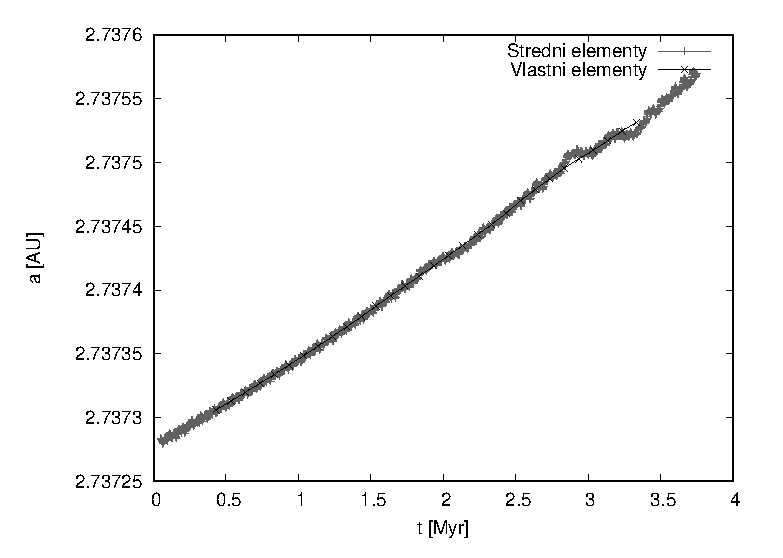
\includegraphics[width=0.8\textwidth]{obr/atFP}
	\caption{Porovnání střední hlavní poloosy $a_{\rm m}$ a~vlastní $a_{\rm p}$ pro simulaci jedné planetky po dobu $3,76$ miliónů let. Lze vidět, že se za tuto dobu vlastní hlavní poloosa planetky zvýšila o~$\Delta a\doteq0.0002\,{\rm AU}\doteq30000\, {\rm km}$. Tento vývoj je způsoben Jarkovského jevem (viz~\ref{sec:jarko}), lze z~grafu vyvodit, že tato planetka měla \I{prográdní} rotaci, neboť se její hlavní poloosa zvětšila.}
	\label{atFP}
\end{figure}

Vlastní elementy jsou elementy dráhy zbavené jak krátkých, tak dlouhých periodických perturbací, mezi které kromě již zmíněných patří navíc sekulární rezonance, které jsou způsobené závislostí frekvencí precese (změny) argumentu perihélia a~délky vzestupného uzlu planetky a~některé jiné planety nebo i~více planet.

Vlastní elementy jsou tedy svým způsobem aritmetickými \uv{průměry} pohybu a~jsou téměř neměnné na dlouhém časovém úseku, ačkoliv působením negravitačních sil --- především zmiňovaného Jarkovského jevu --- se mohou pomalu zvětšovat nebo zmenšovat. 

Mezi vlastní elementy počítáme pouze vlastní hlavní poloosu $a_{\rm p}$, vlastní excentricitu $e_{\rm p}$ a~vlastní inklinaci $i_{\rm p}$. Ostatní elementy nemá cenu uvažovat, protože argument perihélia i~délka vzestupného uzlu periodicky precedují (mění se v~intervalu $0^\circ$ až $360^\circ$) a~střední anomálie je také přibližně lineárně závislá na čase (a~to rychleji).

Výpočet vlastních elementů se provádí pomocí Fourierovy analýzy, viz~\cite{sidlichovsky96}. 

\chapter{Planetky ve~sluneční soustavě} \label{ch:planetky}

\begin{figure}[!htb]
	\centering
	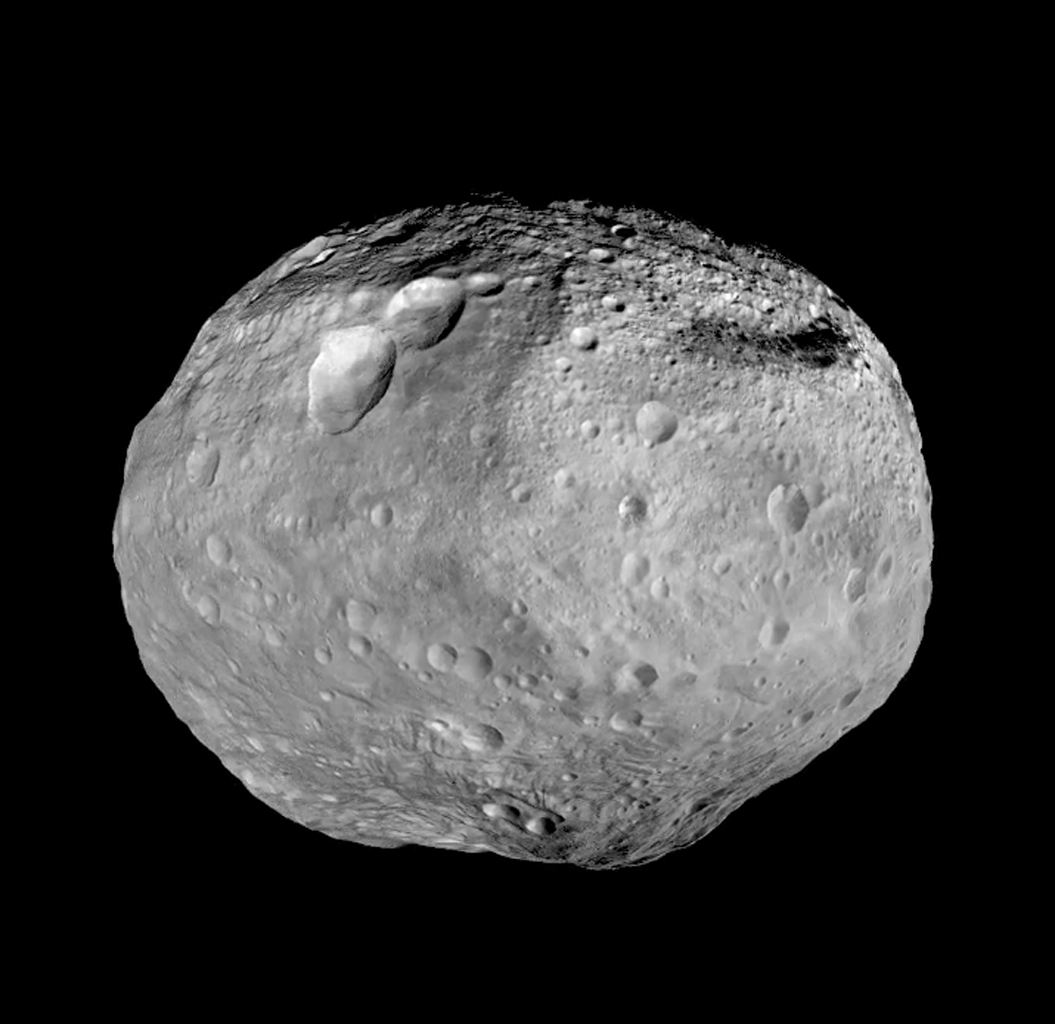
\includegraphics[width=0.6\textwidth]{obr/vesta.jpg}
	\caption{Planetka (4) Vesta, která je po trpasličí planetě (1) Ceres druhým největším a~nejhmotnějším tělesem hlavního pásu planetek. Na jižní hemisféře lze pozorovat kráter Rheasylvia, který je jedním z~největších ve~sluneční soustavě. Fotografie byla pořízena sondou \I{Dawn}, jejímž cílem bylo i~těleso (1) Ceres. Převzato z~\cite{jplvesta}.} \label{fig:vesta}
\end{figure}

Podle Mezinárodní astronomické unie (IAU) se tělesa ve~sluneční soustavě dělí především na planety, trpasličí planety, planetky, komety, přirozené satelity. Planeta je definována jako takové těleso, které obíhá kolem Slunce, není měsíc a~má dostatečnou hmotnost, aby se ustavil přibližně kulovitý tvar a~aby si \uv{vyčisťovalo} svoje okolí od ostatních těles. Kometa je pak těleso složené z~ledu a~prachu, které většinou obíhá Slunce po excentrické dráze, vyhazuje \I{komu} (atmosféru) a~zanechává za sebou \I{ohon}, což je způsobeno sublimací ledu z~komety a~strháváním prachu působením slunečního záření. Další skupinou jsou trpasličí planety, kam v~tuto chvíli patří pouze pět těles: Ceres, Pluto, Eris, Makemake, Haumea. Dále přirozené satelity jsou tělesa obíhající nějaké jiné těleso, různé od Slunce.

Zbývající skupinou jsou planetky (příklad~\ref{fig:vesta}), kam patří transneptunická tělesa (tj.\ obecný název tělesa, která se pohybují za oběžnou dráhou Neptunu), tělesa hlavního pásu planetek a~jiná malá tělesa sluneční soustavy. Planetky můžeme dělit podle jejich oběžné dráhy na tělesa vnitřní a~vnější sluneční soustavy vzhledem k~Jupiteru. Největší populace těles vnitřní soustavy se nachází v~hlavním pásu, který se rozpíná přibližně mezi $2,1\, {\rm AU}$ a~$3,3\, {\rm AU}$ (viz obrázek~\ref{fig:belt}. Dále sem spadají také planetky, jejichž oběžná dráha protíná dráhu Marsu nebo Země --- blízkozemní planetky, a~planetky nacházející se v~libračních bodech L4 a~L5\footnote{To jsou takové body, v~nichž se vyrovnává působení gravitační a~odstředivé síly. Jde tedy o~jakýsi bod rovnováhy. Body L4 a~L5 se nacházejí na oběžné dráze většího tělesa o~$60^\circ$ \uv{napřed} nebo \uv{za} tělesem.} soustav Slunce--Země, Slunce--Mars, Slunce--Jupiter --- tj.\ příslušní Trojáné. Jako Hildy se označují planetky v~rezonanci $3:2$ s~Jupiterem. Dále se předpokládá existence Oortova oblaku, který se má nacházet za hranicí $1\,000\,{\rm AU}$ až do $100\,000\,{\rm AU}$ a~který má být zdrojem dlouhoperiodických komet. Žádné těleso z~této oblasti však ještě nebylo pozorováno.

Většina těles vnější sluneční soustavy se nachází v~Kuiperově pásu, který se sahá od oběžné dráhy Neptunu až do vzdálenosti přibližně $55\, {\rm AU}$. V~nedávné době bylo americkou sondou \I{New Horizons} zblízka prozkoumáno jedno z~těles této oblasti, \I{Ultima Thule}, které je v~tuto chvíli nejvzdálenějším prozkoumaným objektem sluneční soustavy. Jedná se o~dvojité kontaktní těleso (tj.\ má dvě pevně spojené kulovité části), které se zformovalo pravděpodobně při vzniku sluneční soustavy.~\cite{ultimathule}

\pagebreak
\section{Hlavní pás planetek}
Při našem studiu se budeme zaměřovat na planetky hlavního pásu, ve~kterém se také nachází jediná trpasličí planeta ve~vnitřní sluneční soustavě, Ceres, mající střední poloměr $473\, {\rm km}$. Ostatní pozorované planetky mají střední poloměr od několik desítek metrů po $250\, {\rm km}$. Největší populace se rovnoměrně rozprostírá od vzdálenosti $2,1\, {\rm AU}$ od Slunce do vzdálenosti přibližně $3,3\, {\rm AU}$ a~většina planetek má excentricitu menší než $0,4$ a~sklon dráhy menší než $30^\circ$. Planetky, které vystoupí z~této oblasti (ať už zmenšením hlavní poloosy $a$ nebo zvětšením excentricity $e$), se buď přiblíží Marsu, Zemi nebo Venuši a~jsou jejich gravitací vymrštěny na zcela odlišnou oběžnou dráhu, nebo se obdobně přiblíží Jupiteru, který též může výrazně změnit jejich původní oběžnou dráhu nebo může způsobit rozpad tělesa vlivem slapových jevů.

\begin{figure}
	\centering
	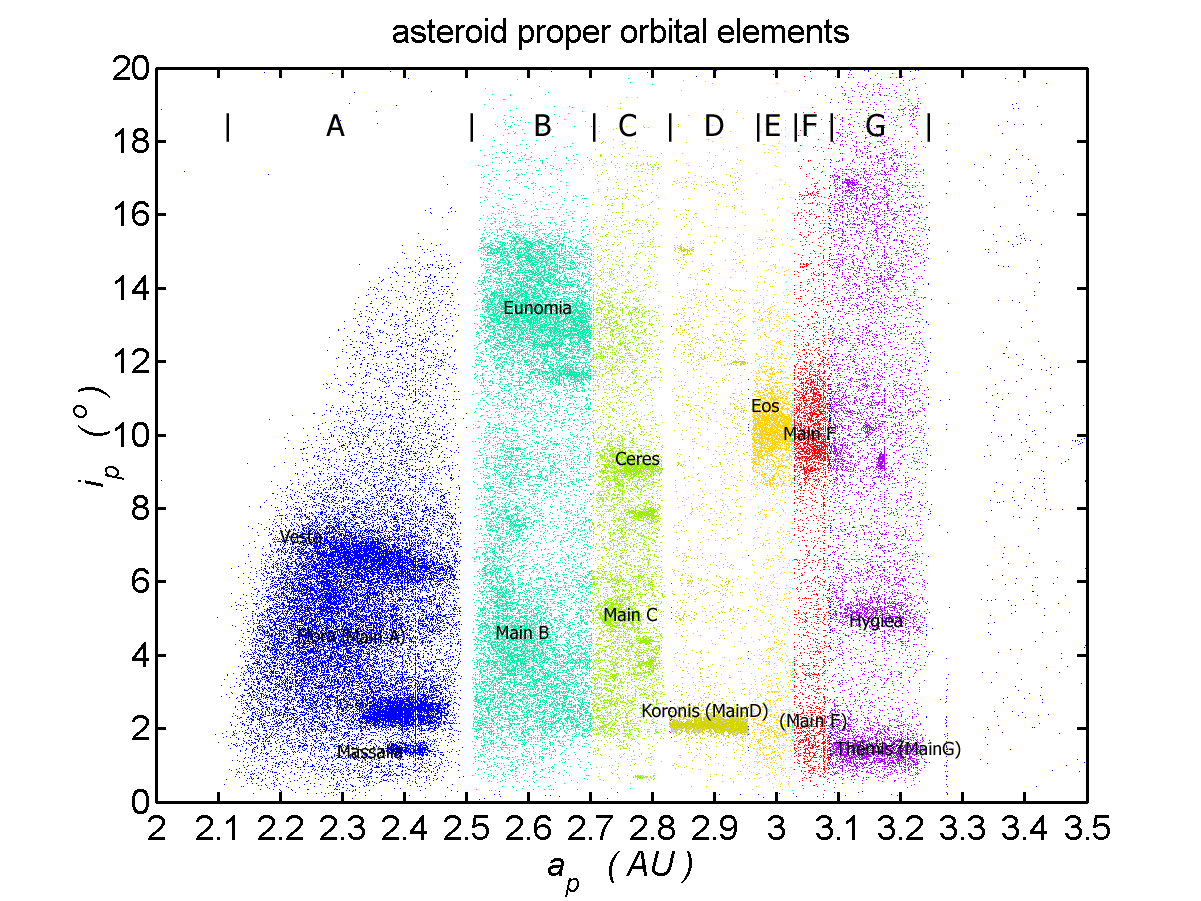
\includegraphics[width=0.9\textwidth]{obr/mainbelt.png}
	\caption{Planetky hlavního pásu podle vlastních elementů --- osa $x$ znázorňuje vlastní hlavní poloosu a~osa $y$ vlastní sklon. Lze vidět některé rodiny planetek, konkrétně uprostřed nahoře se nachází rodina Eunomia. Barevné označení znázorňuje oblasti mezi hlavními rezonancemi středního pohybu. Převzato z~\cite{wiki:belt}.} \label{fig:belt}
\end{figure}

\pagebreak
\section{Rezonance}
Struktura hlavního pásu planetek je významně ovlivněna rezonancemi, které se obecně nachází v~prostoru, ve~kterém když se planetka pohybuje, je nějaký údaj o~její dráze a~o~dráze nějaké planety, běžně Jupitera nebo Saturnu, v~jednoduchém poměru, tedy ve~zlomku s~čita-telem a~jmenovatelem vyjádřenými malými přirozenými čísly. Pro polohy sekulárních rezonancí jsou vztahy podstatně složitější, neboť závisejí na polohách a~hmotnostech více planet.
\subsection{Rezonance středního pohybu} \label{sec:meanmotion}
%Nástin výpočtu jejich polohy (je to jednoduché), vysvětlení vlivu na HCM

Rezonance středního pohybu jsou nejjednodušším a~obvykle také nejsilnějším typem rezonancí. Nastávají, když je oběžná doba planetky a~planety v~poměru malých přirozených čísel, např. $3:2$ --- to znamená, že zatímco planetka dokončí tři celé oběhy, planeta vykoná dva a~obě tělesa se znovu potkají na počáteční pozici. 

Vlivem těchto rezonancí se může hlavní poloosa planetky a~excentricita periodicky měnit, podobně jako je tomu u~kyvadla. Některé rezonance, resp.\ překryvy rezonancí postupně zvyšují excentricitu dráhy planetky, až se její perihélium dostane pod oběžnou dráhu nějaké vnitřní planety, např. Marsu nebo Země, což eventuálně způsobí vzájemné blízké přiblížení, které planetku vymrští na jinou oběžnou dráhu. Takto může planetka úplně opustit sluneční soustavu. Za určitých podmínek se perihélium planetky může snížit natolik, že překročí Rocheovu mez\footnote{což je hraniční vzdálenost od centrálního tělesa, kterou když planetka držená pohromadě pouze vlastní gravitací překročí, je vlivem slapové síly (rozdílu gravitačních sil) roztržena na malé kousky, které jsou soudržné díky elektromagnetickým silám.}, rozpadne se a~úlomky jsou pohlceny hvězdou a~stávají se její součástí~\cite{pichierri17}.

Výpočet umístění rezonance středního pohybu, tedy vzdálenosti od Slunce, je poměrně jednoduchý, uvádíme proto postup pro rezonanci ovlivňující rodinu Eunomia, kterou je rezonance $8:3$ s~Jupiterem. Vzpomeňme na Třetí Keplerův zákon, který říká
\begin{align} \label{eq:3kep}
	\frac{T_1^2}{T_2^2}=\frac{a_1^3}{a_2^3}\,, 
\end{align}
kde $T_1$, $T_2$ označují oběžné doby dvou těles a~$a_1$, $a_2$ jejich hlavní poloosy. Předpokládejme, že v~námi hledané rezonanci $8:3$ se nachází nějaká planetka a~vypočítejme délku její hlavní poloosy, a~to úpravou rovnice~\eqref{eq:3kep} jako
\begin{align} \label{eq:3kepa}
	a_2=\left(\frac{T_2}{T_1}\right)^{\frac{2}{3}}a_1\,,
\end{align}
kde $T_1$, resp.\ $T_2$ zde značí oběžnou dobu Jupitera, resp.\ planetky, a~$a_1$, resp.\ $a_2$ délku hlavní poloosy Jupitera, resp.\ planetky. Oběžná doba Jupitera je přibližně $4332,59\,$dnů a~délka jeho hlavní poloosy přibližně $5,203\,{\rm AU}$. Protože hledáme rezonanci $8:3$, musí platit $\frac{T_2}{T_1}=\frac{3}{8}$. Po dosazení do rovnice~\eqref{eq:3kepa} dostáváme $a_2=2,706\,{\rm AU}$. Tuto rezonanci značenou jako J8/3 lze dobře pozorovat na obrázku~\ref{fig:ae_ai_wise} rozdělení pozorované rodiny Eunomia v~prostoru hlavní poloosy a~excentricity $(a_{\rm p},\,e_{\rm p})$ nebo na obrázku~\ref{fig:ae_sim} simulovaných částic ve~stejném prostoru.
\subsection{Sekulární rezonance} 
Sekulární rezonance jsou sice obvykle mírnějšího rázu než rezonance středního pohybu, ale na dlouhodobý vývoj hlavního pásu mají značný vliv. Slovo sekulární pochází z~latinského \I{saeculum}, což znamená století nebo generace, což odkazuje na dlouhodobý charakter sekulárních rezonancí. Veličiny, které zde dáváme do poměru, jsou rychlosti precese argumentu perihélia $\omega^\prime$ a~rychlosti precese délky vzestupného uzlu $\Omega^\prime$, které ovšem závisejí na hlavní poloose planetky a~jejích vzdálenostech od všech planet. Proto pro jejich polohu neexistuje jednoduchý předpis (viz kap. 7 v~\cite{murray00}).

\pagebreak
\section{Rodiny planetek}

Rodiny planetek jsou skupiny těles, mající podobné charakteristiky, předně podobné vlastní elementy dráhy. Při jejich identifikaci musíme ale přihlížet i~k~ostatním veličinám, jako jsou albedo, barevné indexy, nebo reflexní spektrum.

\immediate\write18{convert -trim obr/trajec_001.png obr/trajec_001t.png}
\immediate\write18{convert -trim obr/trajec_101.png obr/trajec_101t.png}
\immediate\write18{convert -trim obr/trajec_201.png obr/trajec_201t.png}
\immediate\write18{convert -trim obr/trajec_501.png obr/trajec_501t.png}
\begin{figure}
	\centering
	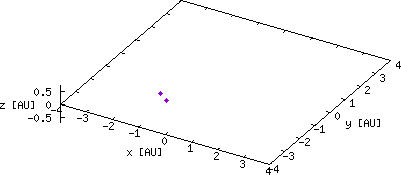
\includegraphics[width=0.49\textwidth]{obr/trajec_001t.png}
	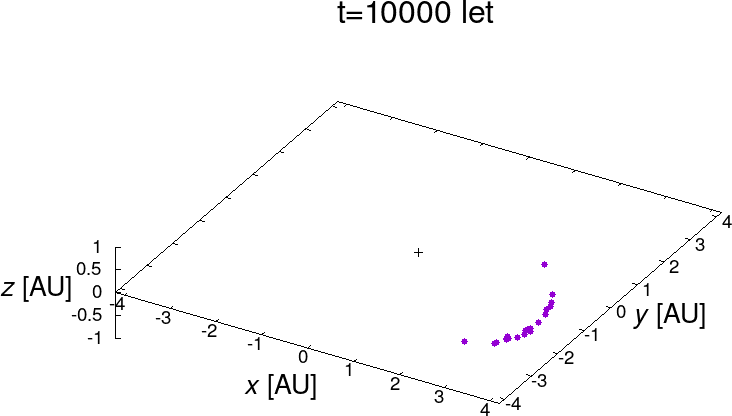
\includegraphics[width=0.49\textwidth]{obr/trajec_101t.png} \\
	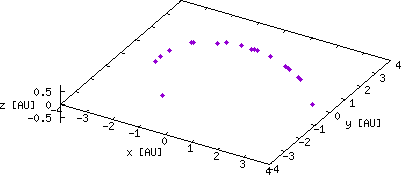
\includegraphics[width=0.49\textwidth]{obr/trajec_201t.png}
	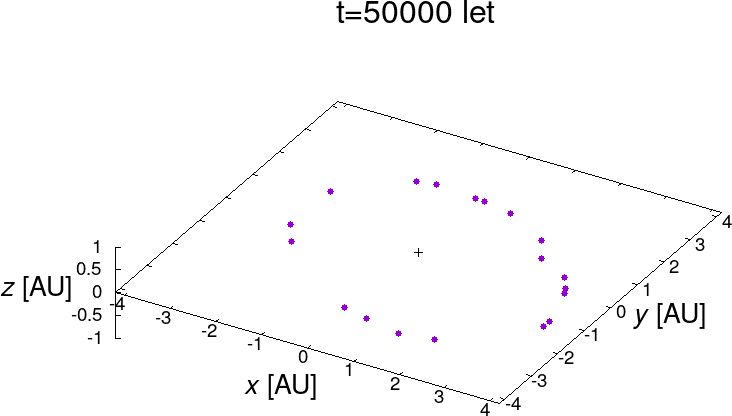
\includegraphics[width=0.49\textwidth]{obr/trajec_501t.png}
	\caption{Trojrozměrné polohy $x,\,y,\,z$ několika těles ($N=20$) ze simulované rodiny Eunomia rušené čtyřmi planetami (Jupiterem, Saturnem, Uranem a~Neptunem) v~časech $t=0,\,10\,000,\,20\,000,\,50\,000\,{\rm let}$ po úvodním izotropním\protect\footnotemark rozpadu. V~čase $t=0$ měla všechna tělesa stejnou polohu $x,\,y,\,z$, ale různé rychlosti $v_x,\,v_y,\,v_z$, tedy i~různé elementy dráhy, především hlavní poloosu, díky čemuž se lišily i~jejich oběžné doby, které se pohybují kolem $4,27$ let. Po $50\,000$ letech lze pozorovat rozprostření podél dráhy ve~střední anomálii $M$, což je element, který je nejsnáze měněn perturbacemi.} \label{fig:trajec}
\end{figure}
\footnotetext{To je takový rozpad, při kterém se tělesa rozletí rovnoměrně do všech směrů.}

Rodiny vznikají srážkou dvou planetek, čemuž v~závislosti na poměru velikosti mateřského tělesa a~projektilu říkáme buď \I{katastrofický rozpad} (\uv{na malé úlomky}), \I{reakumulační rozpad} (úlomky se působením gravitace \uv{slepí} zpátky) nebo \I{kráterování}. Může se zdát, že srážky jsou v~tak rozlehlém prostoru jako je sluneční soustava velmi málo pravděpodobné, ale v~dlouhém časovém úseku --- $4,5\,\text{miliardy let}$ od vzniku naší sluneční soustavy --- k~srážkám dochází, a~mají nejenom vliv na vznik rodin, ale také na jejich následný vývoj (vzniklé fragmenty se spolu nadále srážejí).

Rodiny planetek, které již prošly dlouhodobým vývojem, se samozřejmě na obloze nejeví jako skupina společně letících planetek, kvůli rozdílné hlavní poloose $a$, resp.\ oběžné době $T$ se totiž záhy rozptýlí ve~střední anomálii $M$, jak lze vidět na obrázku~\ref{fig:trajec}.

\subsection{Metody identifikace rodin} \label{sec:metodyiden}
Nejpoužívanější metodou pro identifikaci rodin planetek je \I{hierarchická shlukovací metoda} (HCM) \cite{zappala90}. Spočívá v~tom, že si v~trojrozměrném prostoru vlastních elementů ($a_{\rm p},\,e_{\rm p},\,i_{\rm p}$) zvolíme metriku --- veličinu, kterou budeme popisovat vzdálenost dvou těles, a~poté, pomocí zvolené hraniční \I{vzájemné} vzdálenosti, určíme, která tělesa patří do rodiny. Tato metrika má přitom jednotku rychlosti, aby ji bylo možné porovnávat s~rychlostmi výhozu fragmentů. Je určena vztahem
\begin{align}
	v=na_{\rm p}\sqrt{C_a\left(\frac{\Delta a_{\rm p}}{a_{\rm p}}\right)^2+C_e(\Delta e_{\rm p})^2+C_i(\Delta \sin i_{\rm p})^2}\,,
\end{align}
kde $n$ značí střední pohyb. Dále pokud označíme $1$ a~$2$ tělesa, mezi kterými vzdálenost počítáme, platí $a_{\rm p}=(a_{{\rm p}1}+a_{{\rm p}2})/2$ (kvůli symetrii) a~$\Delta a_{\rm p}=a_{{\rm p}1}-a_{{\rm p}2}$, $\Delta e_{\rm p}=e_{{\rm p}1}-e_{{\rm p}2}$ a~$\Delta \sin i_{\rm p}=\sin i_{{\rm p}1}-\sin i_{{\rm p}2}$; $C_a,\,C_e,\,C_i$ jsou váhy, které přiřazujeme jednotlivým elementům, přičemž možnou a~i~v~této práci použitou volbou je $C_a=5/4$, $C_e=2$, $C_i=2$~\cite{zappala90}. 

Samotný průběh tohoto algoritmu je jednoduchý: zvolíme nějakou hraniční rychlost $v_{\rm cutoff}$ a~poté, většinou počínaje největším tělesem, např. (15) Eunomia, hledáme dvojice těles, pro které je $v<v_{\rm cutoff}$; vždy když nějakou nalezneme, přidáme si ji do seznamu zkoumané rodiny a~postup opakujeme, dokud nám nepřibývají žádní noví členové. Výsledný počet členů je samozřejmě závislý na volbě $v_{\rm cutoff}$, což lze vidět na obrázku~\ref{fig:Nv}.

Jak ukážeme později v~této práci (kap.~\ref{sec:interlopers}), tato metoda samotná nestačí ke kompletní identifikaci rodiny, neboť musíme odstranit \I{přimísená tělesa} (angl.\ interlopers), např.\ porovnáním albed (viz obrázek~\ref{fig:pV_pIR}), barevných indexů (viz obrázek~\ref{fig:astar_iz}), grafu závislosti hlavní poloosy a~hvězdné velikosti, případně dalšími metodami závisejícími na konkrétní situaci v~okolí rodiny.

\subsection{Nevratné děje při vývoji}
%Disipační síly, vliv na vývoj v~prostoru vlastních elementů, reference na nějaký článek o~nové databázi tvarů planetek???

Dosud jsme se zabývali pouze silami, které vznikají vzájemným gravitačním působením těles, ve~sluneční soustavě ale působí i~několik dalších sil, týkajících se zejména emise tepla. Společně s~náhodnými srážkami a~chaotickou difuzí tvoří tyto jevy nevratné děje při vývoji planetek a~komet, se kterými je při jejich studiu nutno počítat.

\subsubsection{Jarkovského jev} \label{sec:jarko}
Jarkovského jev, který je pojmenován po Ivanu Ospichovi Jarkovském\footnote{Jarkovský ale tento jev nepopsal úplně stejně, jako ho chápeme teď; v~tehdejší době byla ještě populární teorie o~éteru --- všudypřítomném médiu --- a~právě této látce Jarkovský připisoval ono zpomalování nebo zrychlování těles. Tento jev v~dnešním pojetím popsali nezávisle Ernst Julius Öpik (1893--1985) a~Vladimir Vyacheslavovich Radzievskii (1911--2003)~\cite{brozphd}.}  (1844--1902), je nejdůležitější negravitační silou, která ovlivňuje strukturu hlavního pásu planetek. Jejím působením se totiž tělesa posouvají v~hlavní poloose, čímž se dostávají do oblastí rezonancí, které pak mohou jejich pohyb nadále ovlivnit.

\begin{figure} 
	\centering

		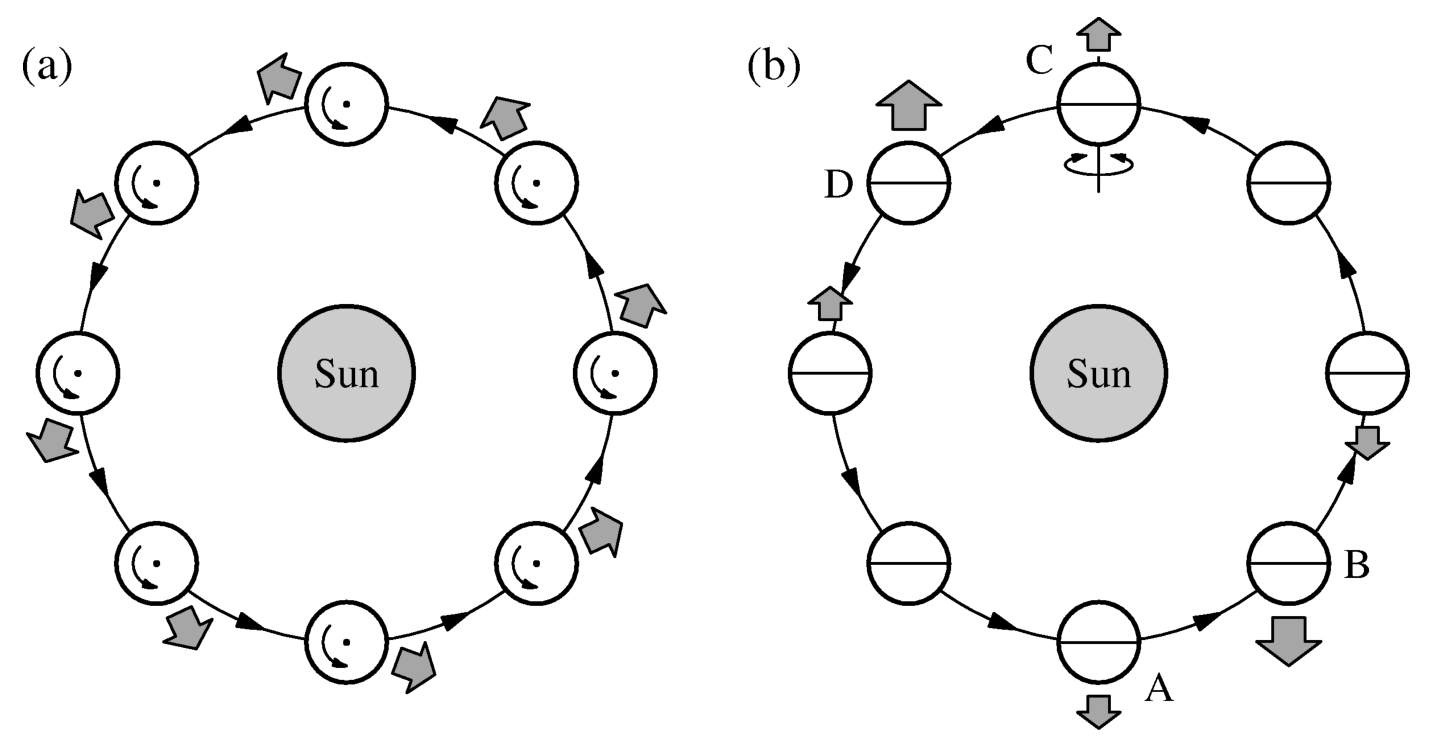
\includegraphics[width=0.8\textwidth]{obr/jarkovskeho_jev.png}
	\caption{Denní a~roční varianta Jarkovského jevu. Šedivé šipky
	označují zbytkovou sílu, která působí na těleso. (a) Denní Jarkovského jev, když se těleso otáčí kolem osy kolmé k~oběžné dráze. V~tomto případě se těleso natočí teplejší stranou vždy \uv{za sebe}, tepelnou emisí pak vzniká zbytková síla, jejíž jedna složka působí ve~směru pohybu tělesa, hlavní poloosa se tedy bude zvětšovat. (b) Roční Jarkovského jev, s~rotační osou ležící v~orbitální rovině. Ohřívání přivrácené polokoule, zejména v~bodech A~a~C, a~opožděná emise tepelného záření, zvláště v~bodě B a~D, způsobují zbytkovou sílu, jejíž jedna složka směřuje proti pohybu tělesa, tudíž hlavní poloosa se bude zmenšovat. Převzato z~\cite{fmt}.} \label{fig:jarko}
\end{figure}

Rozlišujeme dvě varianty Jarkovského jevu --- denní a~roční. Jejich rozdíl je popsán v~\ref{fig:jarko}. Výsledná změna hlavní poloosy je samozřejmě důsledkem kombinace obou variant, pro tělesa s~hodnotou šikmosti (obliquity)\footnote{Obliquita je úhel mezi rotační osou tělesa a~kolmicí k~dráze, obliquita $0^\circ$ a~$180^\circ$ značí rotační osu kolmou na ekliptiku, přičemž $0^\circ$ je tzv.\ prográdní rotace (těleso vlivem Jarkovského efektu zrychluje) a~$180^\circ$ tzv.\ retrográdní rotace (těleso zpomaluje).} blízko $0^\circ$ nebo $180^\circ$ dominuje denní varianta, zatímco pro obliquitu kolem $90^\circ$ je roční varianta silnější. Dále pro tělesa s~rychlejší rotační periodou (řádově menší než oběžná doba) je silnější denní varianta, a~pro tělesa s~delší rotační periodou roční varianta. 

Jarkovského jev byl poprvé pomocí radarů změřen v~roce 2003 při zkoumání pohybu blízko-zemní planetky (6489) Golevka.~\cite{chesley03}
\subsubsection{YORP jev}
%Popis,  zesílení Jarkovského jevu

Yarkovsky–O'Keefe–Radzievskii–Paddack jev je stejně jako Jarkovského jev důsledkem nerovnoměrného rozložení a~emise tepla tělesa, YORP však funguje pouze pro nesférická tělesa. Jeho účinkem je zvětšování úhlové rychlosti rotace $\omega$ a~zmenšování obliquity $\theta$ a~je způsoben nepravidelným povrchem planetky, který vyzařuje teplo nerovnoměrně. V~dlouhém časovém měřítku YORP \enquote{táhne} úhlovou rychlost buď k~$0$, nebo k~nekonečnu a~obliquitu buď ke $0^\circ$ nebo ke $180^\circ$. Protože Jarkovského jev je nejsilnější právě pro tyto hodnoty obliquity, funguje YORP jako takový \uv{zesilovač} Jarkovského jevu. 

Jak YORP, tak Jarkovského jev je silnější pro menší tělesa. Na ty úplně nejmenší tělesa, prachové částice, působí \I{Poynting-Robertsonův efekt}\footnote{Vzájemný pohyb částice a~Slunce způsobuje, že sluneční záření dopadá na částici pod úhlem jiným než $90^\circ$ vzhledem k~pohybu částice, čímž částici zpomaluje.}, který způsobuje postupné zpomalování částice až dojde ke kolizi se Sluncem samotným. 

\subsubsection{Náhodné srážky}
Po úvodní srážce se tělesa zpět reakumulují do větších kusů, které nadále letí po heliocentrických drahách, a~je zřejmé, že v~dlouhém časovém úseku se některá z~nich srazí s~nějakým jiným tělesem. Tím vznikají další menší tělesa, jejichž rotační osa a~doba je navíc různá od původního tělesa, což má vliv na Jarkovského a~YORP jev. 

\subsubsection{Chaotická difuze}
Je známo, že dvojité (i~vícenásobné) kyvadlo se chová chaoticky, tedy jeho stav je velmi náchylný k~drobným změnám počátečních podmínek. To ale neznamená, že jeho vývoj nemůžeme simulovat, jedná se totiž o~\I{deterministický chaos}. Jak jsme zmiňovali v~\ref{sec:meanmotion}, dráhové rezonance se chovají podobně jako kyvadlo, a~proto, když se rodina nachází blízko překryvu dvou nebo více rezonancí, mohou někteří její členové tuto oblast chaoticky opustit. Tento děj je v~podstatě nevratný, protože takový chaotický systém nelze rozumně zpětně integrovat.

\chapter{Vlastnosti rodiny Eunomia} \label{ch:eunomia}
% Postup určování rodiny, volba $v_{cutoff}$, pozadí --- [česky???] interlopers (ref na později), rozdělení velikostí 
Rodina Eunomia se nachází v~centrálním pásu planetek --- mezi $2,5\,{\rm AU}$ a~$2,82\,{\rm AU}$ --- a~patří mezi nejpočetnější rodiny vůbec~\cite{nesvorny15}. Její členové včetně největšího tělesa jsou taxonomického typu S, což znamená, že mají červené reflekční spektrum s~absorpčním pásem na $9\,{\rm mm}$ a~že se převážně skládají z~křemičitanů. Existují hypotézy, že původní mateřské těleso nebylo homogenní, ale částečně diferenciované~\cite{nathues05}, což by mohlo znamenat určité zvýšení počtu členů této rodiny, neboť bychom mezi členy mohli zahrnout i~tělesa odlišná typu S.

V~rámci ucelené analýzy rodiny Eunomia jsme nejprve pomocí algoritmu HCM znovu identifikovali její členy dle nových observačních dat a~poté určili pravděpodobné místo rozpadu (tzn. hodnoty $f$ a~$\omega + f$). Následně jsme vytvořili izotropní rychlostní pole rozpadu, ze kterého jsme v~kombinaci s~pozorovanými průměry a~předpokládanými hustotami planetek vytvořili syntetickou populaci 6210 testovacích částic, které jsme pak simulovali po dobu jedné miliardy let a~výsledky pak porovnali s~pozorovanou rodinou.

\newpage
\section{Identifikace členů}

Jak již bylo naznačeno, v~této práci jsme k~prvotní identifikaci členů rodiny Eunomia použili \textit{hierarchickou shlukovací metodu}, popsanou v~části~\ref{sec:metodyiden}. Závislost počtu členů rodiny na hraniční rychlosti lze vidět na obrázku~\ref{fig:Nv}. Můžeme pozorovat, že rodina Eunomia je poměrně zřetelně oddělená od ostatních rodin --- jedinou blízkou rodinou je rodina Adeona, jejíž planetky ovšem nejsou součástí rodiny Eunomia. K~dalším výpočtům jsme použili hodnotu $v_{\rm cutoff}=44\,{\rm m/s}$, při které počet členů rodiny před odstraněním přimísených těles činil 6503.

\begin{figure}
	\centering
	\includegraphics[width=0.6\textwidth]{obr/Nv}
	\caption{Závislost počtu členů rodiny Eunomia na zvolené hraniční rychlosti $v_{\rm cutoff}$ při použití metody HCM. Počet členů prudce vzroste při přechodu z~rychlosti $43\,{\rm m/s}$ na $44\,{\rm m/s}$, což je způsobené poměrně velkou vzdáleností prvního nejbližšího tělesa od mateřského (15) Eunomia. Dále vzroste prudce při přechodu z~rychlosti $46\,{\rm m/s}$ na $47\,{\rm m/s}$, což je způsobené splynutím s~rodinou Adeona.}
	\label{fig:Nv}
\end{figure}

\subsection{Přimísená tělesa} \label{sec:interlopers}
%Odstranění interlopers, barevné indexy, SLOAN, WISE, ref na Nejistoty veřejných dat.

\subsubsection{Graf $(a_{\rm p},\,H)$}


Prvním mechanismem k~odstranění přimísených těles je závislost unášení ve~vlastní hlavní poloose $\Delta a_{\rm p}$ na~\textit{absolutní hvězdné velikosti} $H$\footnote{\textit{Absolutní hvězdná velikost} neboli \textit{magnituda} $H$ je pro planetky ve~sluneční soustavě taková \textit{zjevná hvězdná velikost}, kterou by planetka měla, kdyby byla vzdálená $1\,{\rm AU}$ od Slunce a~$1\,{\rm AU}$ od Země a~fázový úhel Slunce--planetka--Země činil $0^\circ$. V~podstatě to znamená, že se na planetku díváme \uv{ze středu Slunce}. Planetka s~průměrem $1\,{\rm km}$ a~albedem $p_{\rm V}=1$ má statisticky $H=15,648\,{\rm mag}$. Pro \textit{absolutní hvězdné velikosti} obecně platí Pogsonova rovnice, která popisuje relativní vztah \textit{magnitud} dvou těles
\begin{align*}
	H_2-H_1=-2,5\log\left(\frac{L_2}{L_1}\right)\,,
\end{align*}
kde $L_1$, resp. $L_2$ označují zářivé výkony těles.}
(obrázek~\ref{fig:aH_wise}), způsobená vlivem Jarkovského jevu a~YORPu. Platí, že unášení v~hlavní poloose (též zrychlení) je větší pro menší tělesa, protože obsah povrchu planetky, kterému je úměrná Jarkovského síla, roste s~druhou mocninou poloměru, zatímco objem, kterému je úměrná hmotnost, roste s~třetí mocninou poloměru. Tím lze odstranit tělesa, která se vzhledem k~jejich hvězdné velikosti nemohla unášením po původním rozpadu dostat na grafu $(a_{\rm p},\,H)$ tam, kde jsou. Tuto závislost lze modelovat funkcí 
\begin{align}
	H=5\log\left(\frac{\Delta a_{\rm p}}{C}\right)\,,
\end{align}

\begin{figure}
	\centering
	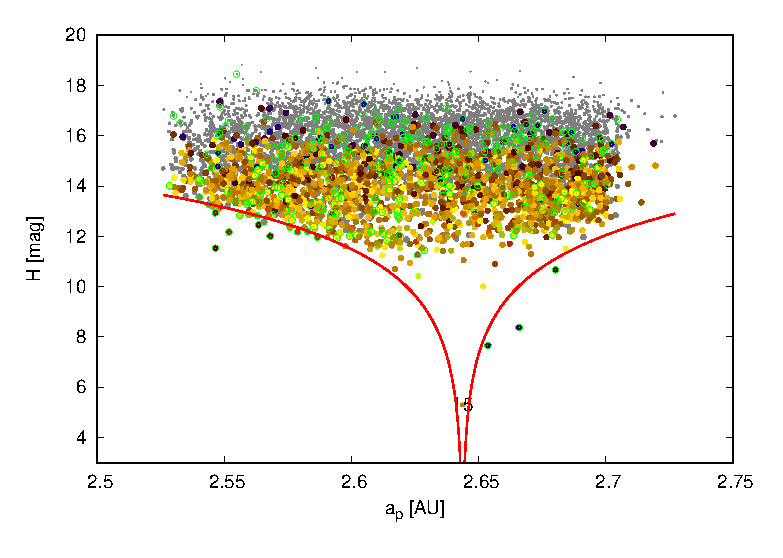
\includegraphics[width=0.7\textwidth]{obr/aH_wise}
	\caption{Rozdělení pozorované rodiny Eunomia v~rovině vlastní hlavní poloosy $a_{\rm p}$ a~absolutní hvězdné velikosti $H$. Barevná škála byla zvolnea dle~katalogu WISE. Šedá křivka označuje funkci s~parametry ${C=2,2\cdot10^{-4}}$ a~${a_{\rm c}=2,643666\,{\rm AU}}$ a~červená křivka označuje posunutou funkci s~parametry ${C=2\cdot10^{-4}}$ a~${a_{\rm c}=2,641666\,{\rm AU}}$. K~odstranění  jsme zvolili červenou funkci. Lze pozorovat typický tvar \uv{V}, který je způsobem počátečním rychlostním polem a~Jarkovského jevem, jenž je ještě zesílen vlivem YORPu, což způsobuje zvýšenou koncentraci malých planetek při okrajích rodiny.}
	\label{fig:aH_wise}
\end{figure}

kde $H$ označuje absolutní magnitudu, $\Delta a_{\rm p}$ vzdálenost v~hlavní poloose od středu rodiny a~$C$ parametr, který záleží na naší volbě. Běžně se jako střed rodiny bere největší těleso, v~našem případě jsme ale byli nuceni celou funkci o~něco posunout, aby lépe odpovídala ostatním pozorovaným objektům. Zvolené hodnoty lze najít v~popisku obrázku~\ref{fig:aH_wise}.

\subsubsection{Graf $(p_{\rm V},\,p_{\rm IR})$ a~$(a^*,\,i-z)$}

\begin{figure}
	\centering
	\includegraphics[width=0.9\textwidth]{obr/pV_pIR}
	\caption{Albeda $p_{\rm V}$ (ve viditelném spektru) a~$p_{\rm IR}$ (v~infračerveném spektru) z~katalogu WISE \cite{nugent15}. Barevná škála byla taktéž převzata z~katalogu WISE, barvy neodpovídají reálnému zbarvení. Zelené kroužky označují přimísená tělesa vyřazená jakoukoliv z~použitých metod. Pro vyřazení přimísených těles touto metodou byly zvoleny hraniční hodnoty $0,05 \leq p_{\rm V} \leq 0,4$.}
	\label{fig:pV_pIR}
\end{figure}

Další metodou k~odstranění přimísených těles jsou metody spektroskopické, tedy zkoumající odrazivé charakteristiky těles. První z~nich je graf závislosti albed\footnote{Geometrické albedo je poměr zářivosti tělesa ku zářivosti ideálního bezztrátového disku o~stejném průřezu.~\cite{fmt}} ve~viditelném $p_{\rm V}$, resp. v~infračerveném $p_{\rm IR}$ oboru. Pokud uvažujeme, že původní těleso bylo homogenní, měly by vzniklé úlomky mít podobná albeda, čímž lze vyřadit tělesa, která očividně nemohla vzniknout ze stejné mateřské planetky. Závislost $(p_{\rm V},\,p_{\rm IR}$) lze vidět na obrázku~\ref{fig:pV_pIR}, v~jehož popisku lze také najít krajní hodnoty, které jsme volili pouze pro albedo $p_{\rm V}$, protože albedo $p_{\rm IR}$ je mu často přímo úměrné.


Podobně můžeme identifikovat přimísená tělesa pomocí jejich barevných indexů $a^*$ a~$i-z$, tentokrát z~katalogu SDSS (Sloan Digital Sky Survey), který používá fotometrický systém skládající se z~pěti filtrů $u,\,g,\,r,\,i,\,z$, přičemž každý z~nich propouští světlo o~daném rozsahu vlnových délek. Zmíněné veličiny $u,\,g,\,r,\,i,\,z$ pak označují zjevnou jasnost (v~magnitudách). Veličina $a^*$ je definována vztahem~\cite{ivezic01}
\begin{align}
	a^ *= 0,89 (g - r) + 0,45 (r - i) - 0,57\,.
\end{align}

\begin{figure}
	\centering
	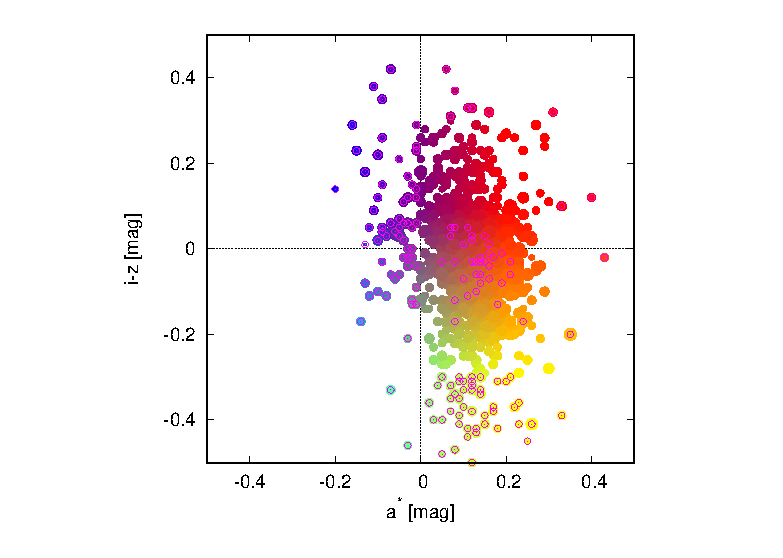
\includegraphics[width=0.9\textwidth]{obr/astar_iz}
	\caption{Barevné indexy $a^*$ a~$i-z$ z~katalogu Sloan \cite{ivezic01}. Barevná škála byla taktéž zvolena dle~katalogu Sloan, barvy neodpovídají reálnému zbarvení. Zelené kroužky označují přimísená tělesa vyřazená jakoukoliv z~použitých metod. Pro vyřazení přimísených těles byly zvoleny hraniční hodnoty $0\leq a^* \leq 0,3$ a~$-0,3\leq i-z \leq 0,3$.}
	\label{fig:astar_iz}
\end{figure}

Zvolené krajní hodnoty lze nalézt v~popisku obrázku~\ref{fig:astar_iz}. 

Celkový počet vyřazených těles po použití všech metod činil 319 a~počet členů pozorované rodiny Eunomia pro $v_{\rm cutoff}=44\,{\rm m/s}$, se kterou pracujeme v~dalších výpočtech, činil 6184.

\pagebreak

\section{Fyzikální model pro rodinu Eunomia}
%Rozdělení v~$ae$ a $ai$ prostoru, vliv rezonancí J8/3 a J13/5, Gaussovy rovnice --- elipsa, volba bodu rozpadu ($f=90^o$, $\omega+f=50^o$).
V~následující části vytvoříme fyzikální model pozorované rodiny Eunomia identifikované v~předchozí části, který budeme později porovnávat s~výsledky simulace orbitálního vývoje.
\subsection{Rozdělení velikostí}
\begin{figure}
	\centering
	\begin{subfigure}[b]{0.45\textwidth}
	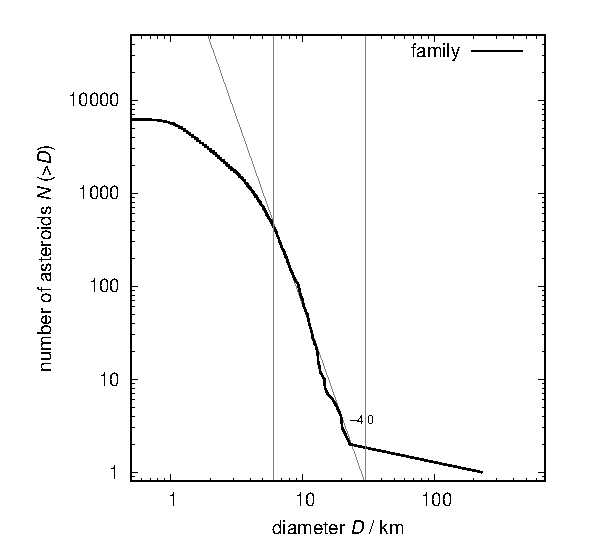
\includegraphics[width=\textwidth]{obr/size_distribution}
	\end{subfigure}
	\begin{subfigure}[b]{0.45\textwidth}
	\includegraphics[width=\textwidth]{obr/size_distribution_SMALLD}
	\end{subfigure}
	\caption{Histogram četnosti velikostí planetek rodiny Eunomia pro $v_{\rm cutoff}=44\,{\rm m/s}$, kde veličina $N({>}D)$ označuje počet planetek s~průměrem větším než $D$. Jedná se o~logaritmický graf $(\log D,\,\log N({>}D))$, na kterém lze vztah mezi danými veličinami aproximovat přímkou, což znamená, že vztah mezi veličinami $D$ a~$N({>}D)$ je mocninný. Vodorovná část zcela vlevo je způsobena observační nedostatečností.}
	\label{fig:sfd}
\end{figure}

Jednou ze základních charakteristik rodiny planetek je její rozdělení velikostí, pro rodinu Eunomia jej můžeme vidět na obrázku~\ref{fig:sfd}. Změna sklonu přímky prvního intervalu $D$ (vlevo, $q=-4$) na druhý interval $D$ (vpravo, $q=-1,2$) je důsledkem jednak prvotního rozpadu a~jednak druhotného vývoje. Rozdělení velikostí se samozřejmě mění s~časem --- tělesa se nadále srážejí, vytvářejí menší tělesa, která snáze opouštějí rodinu (např. působením rezonancí, Jarkovského jevu nebo i~Poyntingova-Robertsonova efektu).

Při vytváření syntetické populace planetek je nutné toto rozdělení velikostí zohlednit. Při přiřazování průměrů simulovaným částicím jsme proto použili přímo rozdělení velikostí pozorované rodiny Eunomia. Při zpracovávání simulace jsme rozdělení korigovali tak, aby odpovídalo pozorovanému.

\subsection{Rozdělení v~prostoru $(a_{\rm p},\,e_{\rm p},\,\sin I_{\rm p})$}
\begin{figure}
	\centering
	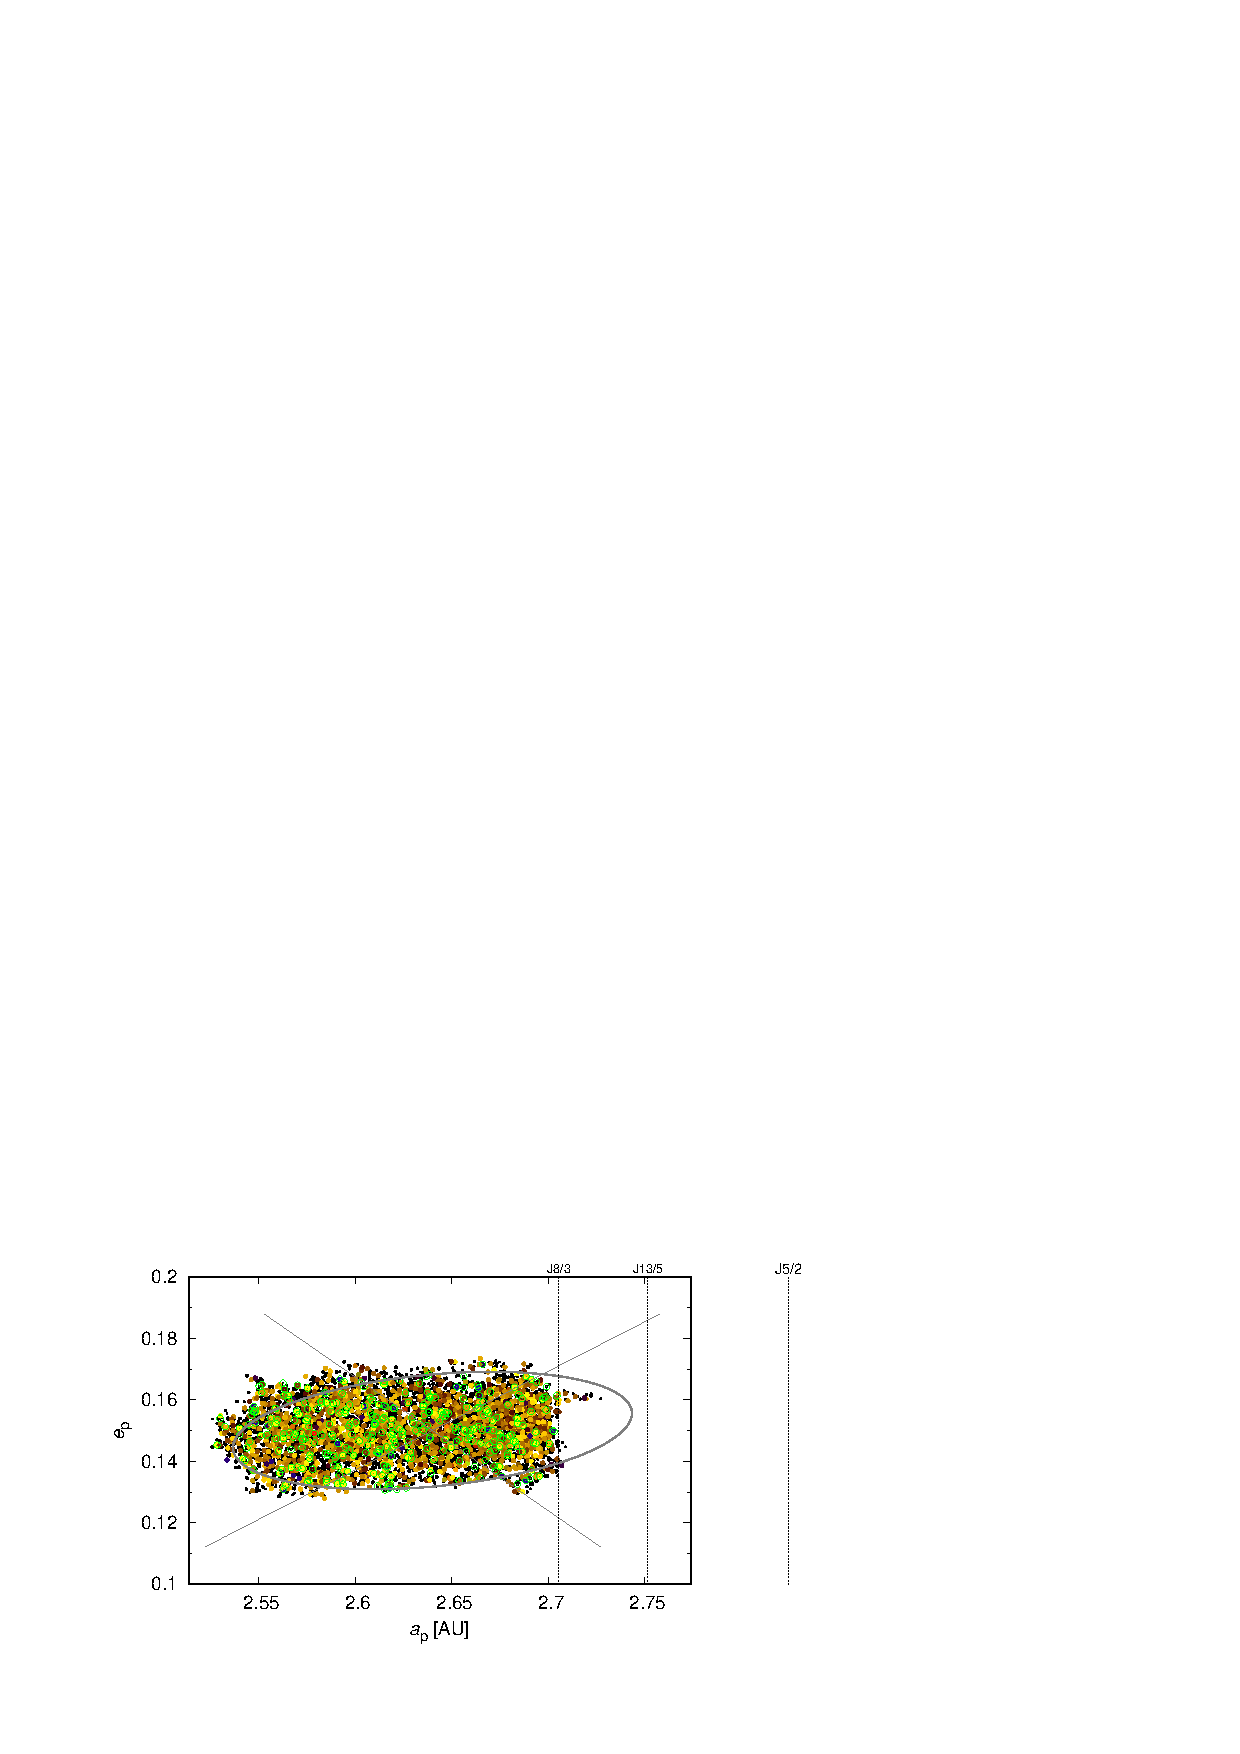
\includegraphics[width=0.8\textwidth]{obr/ae_wise}
	\includegraphics[width=0.8\textwidth]{obr/ai_wise}
	\caption{Pozorovaná rodina Eunomia pro hraniční rychlost $v_{\rm cutoff} = 44\,{\rm m/s}$ v~rovině vlastní hlavní poloosy $a_{\rm p}$ a~vlastní excentricity $e_{\rm p}$ (nahoře) a~v~rovině vlastní hlavní poloosy $a_{\rm p}$ a~vlastního sklonu $\sin I_{\rm p}$ (dole). Barevná škála odpovídá albedu $p_{\rm V}$ a~$p_{\rm IR}$ z~katalogu WISE\@. Nápisy J8/3 a~J13/5 označují polohu rezonancí středního pohybu s~Jupiterem. Šedé elipsy a~úsečky (degenerované elipsy) naznačují výpočet Gaussových rovnic pro hodnoty pravé anomálie $f=0^\circ,\,90^\circ,\,180^\circ$ (nahoře) a~součtu $\omega+f=0^\circ,\, 50^\circ,\, 90^\circ$ (dole), kde zvolenou tučnější elipsou je elipsa pro hodnoty $f=90^\circ$ a~$\omega+f=50^\circ$.}
	\label{fig:ae_ai_wise}
\end{figure}

Jedním z~nejdůležitějších úkonů, které je nutno provést před spuštěním simulace orbitálního vývoje, je určit, kde nastal úvodní rozpad (tzn. zvolit hodnoty pravé anomálie $f$ a~součtu argumentu pericentra s~pravou anomálií $\omega+f$), to totiž může významně ovlivnit rozdělení rodiny na grafech vlastní hlavní poloosy $a_{\rm p}$ versus vlastní excentricita $e_{\rm p}$ (prostor $(a_{\rm p},\,e_{\rm p})$) nebo versus vlastní sklon $\sin I_{\rm p}$ (prostor $(a_{\rm p},\,\sin I_{\rm p})$). Na obrázku~\ref{fig:ae_ai_wise} můžeme vidět pozorovanou rodinu Eunomia společně s~elipsami, které korespondují s~rozdělením rodiny při rozpadu na různých místech. Tyto elipsy jsou určeny Gaussovými rovnicemi: pokud na těleso na začátku působí zrychlení $\vec{a}=(R,\,T,\,W)$, kde $R$ označuje radiální složku (podél spojnice s~centrálním tělesem), $T$ transverzální složku (podél tečny k~oběžné dráze po směru oběhu) a~$W$ normálovou složku (kolmou na rovinu oběhu), budou se elementy dráhy tělesa měnit jako~\cite{fmt}
\begin{align}
	\diff{a}{t}&=\frac{2}{n\sqrt{1-e^2}}\left[T+e(T\cos f+R\sin f)\right] \,, \\
	\diff{e}{t}&=\frac{\sqrt{1-e^2}}{na}\left[R\sin f+T(\cos f+\cos E)\right]\,, \\
	\diff{I}{t}&=\frac{W}{na\sqrt{1-e^2}}\frac{r}{a}\cos(\omega+f)\,,
\end{align}
kde $a$ označuje hlavní poloosu, $e$ excentricitu, $I$ sklon, $n$ střední pohyb, $f$ pravou anomálii, $E$ excentrickou anomálii (viz obrázek~\ref{fig:E}), $\omega$ argument pericentra (viz obrázek~\ref{fig:elip}) a~$r$~vzdálenost od centrálního tělesa.

Jak můžeme vidět v~Gaussových rovnicích i~na obrázku~\ref{fig:ae_ai_wise}, na hlavní poloosu a~excentricitu má vliv pouze hodnota $f$, zatímco na sklon má vliv pouze hodnota $\omega+f$. Vizuálním porovnáním s~pozorovanou rodinou v~prostorech $(a_{\rm p},\,e_{\rm p})$ a~$(a_{\rm p},\,\sin I_{\rm p})$ jsme zvolili hodnoty $f=90^\circ$ a~$\omega+f=50^\circ$.

\newpage
\section{Simulace orbitálního vývoje}

Konečně se dostáváme k~části, kde budeme simulovat dlouhodobý vývoj rodiny Eunomia. Krátkodobý výpočet problému $N$ těles byl již proveden k~vytvoření obrázku~\ref{fig:trajec}, nicméně takový výpočet neříká nic zajímavého o~dynamické struktuře rodiny Eunomia, která se začne projevovat až po miliónech let. Ideálně se musí rodina simulovat po dobu čtyř, miliard let a~posléze analyzovat její vzhled v~prostoru $(a_{\rm p},\,e_{\rm p},\,\sin I_{\rm p})$, včetně jejího rozdělení velikostí. V~našem případě jsme se z~výpočetních důvodů omezili na simulaci rodiny pouze po jednu miliardu let.

%Popis experimentu (údaje o~výpočetní technice)
Pro dlouhodobou simulaci používáme upravený balíček SWIFT \cite{levison94}, s~přidanými výpočty pro denní i~roční Jarkovského jev, YORP efekt, náhodné srážky (kolizní reorientace os), úbytek hmoty způsobený otáčením tělesa a~digitálními filtry k~výpočtu středních a~vlastních elementů (viz kap.~\ref{sec:orbelem}). Úpravy jsou popsány v~\cite{broz11}.

Simulace byla spuštěna na výpočetním clusteru Astronomického ústavu Univerzity Karlovy. Úlohu jsme rozdělili na 32 procesorů; každý prováděl výpočet 200 testovacích částic. Výpočet běžel dosud 30 dní, tzn. že jsme spotřebovali $32\cdot30\cdot24=23040$ CPU hodin. Protože jsme z~ladících důvodů nechali ukládat nejen vlastní, ale i~střední elementy, je celkový objem binárních dat roven $164\,{\rm GB}$.

Bohužel jsme byli nuceni některé skupiny částic restartovat po výpadku proudu, což způsobilo úbytek přibližně poloviny částic kolem $500$ milionů let. Přesto jsme ale získali hodnotná data, která nám například umožní rozhodnout, zda-li nelze rodinu Eunomia vysvětlit jako mladou rodinu.

\newpage
\section{Porovnání simulace a~pozorování}

\immediate\write18{convert -trim obr/ae_5.png obr/ae_5t.png}
\immediate\write18{convert -trim obr/ae_105.png obr/ae_105t.png}
\immediate\write18{convert -trim obr/ae_405.png obr/ae_405t.png}
\immediate\write18{convert -trim obr/ae_905.png obr/ae_905t.png}
\begin{figure}[t]
	\centering
	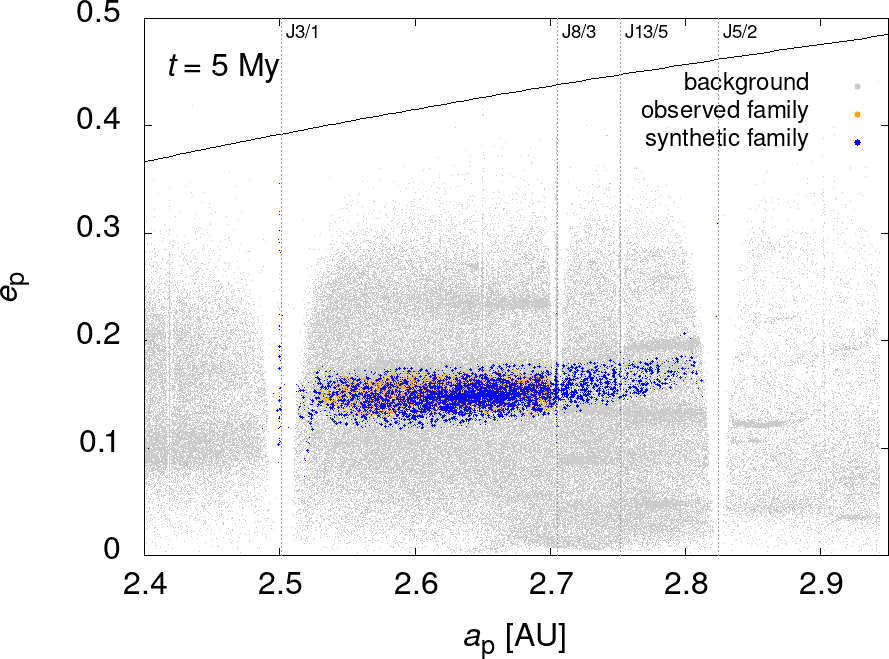
\includegraphics[width=0.49\textwidth]{obr/ae_5t.png}
	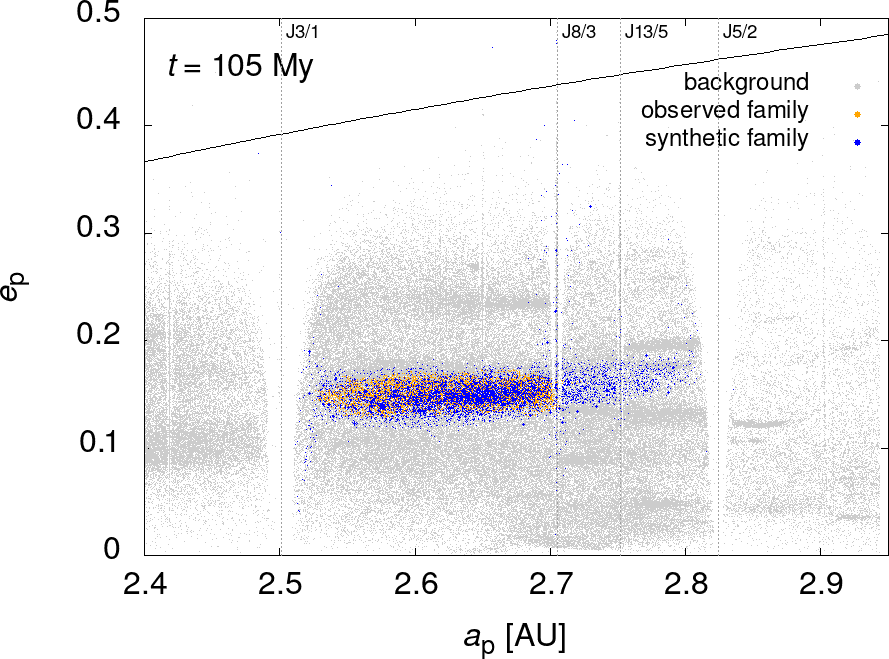
\includegraphics[width=0.49\textwidth]{obr/ae_105t.png}\\
	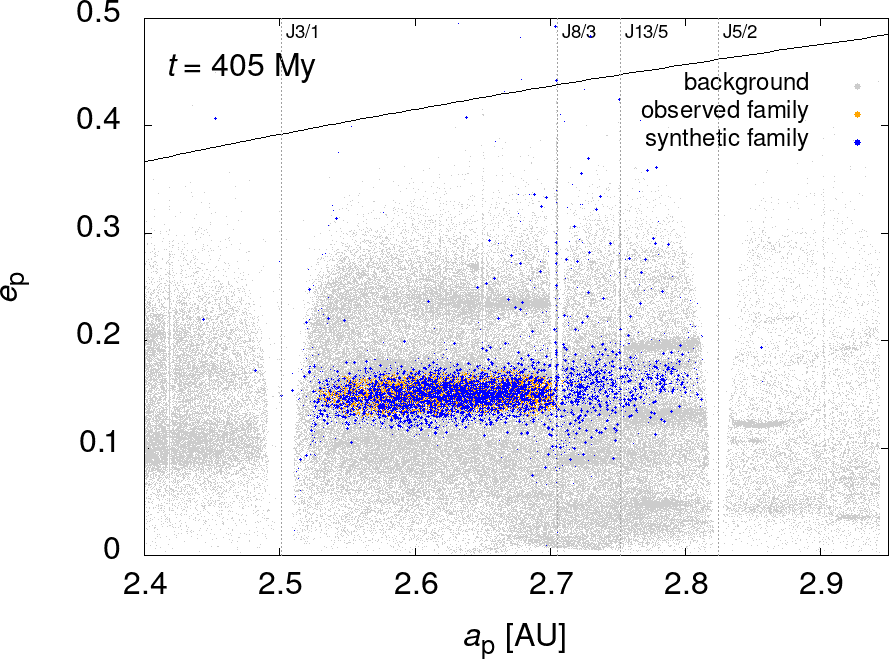
\includegraphics[width=0.49\textwidth]{obr/ae_405t.png}
	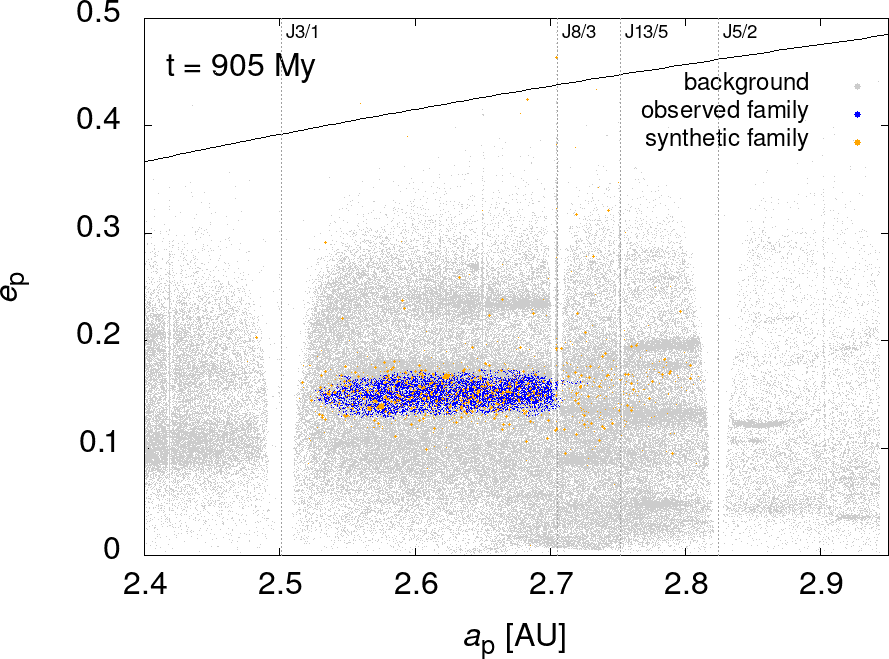
\includegraphics[width=0.49\textwidth]{obr/ae_905t.png}
	\caption{Výsledky simulace v~prostoru $(a_{\rm p},\,e_{\rm p})$ v~časech postupně $t=5,\,105,\,405,\,905$ miliónů let. Modré body označují simulovanou rodinu, žluté body pozorovanou rodinu identifikovanou HCM a~šedé body pozadí a~jiné okolní rodiny. Jsou také značeny nejvýznamnější rezonance s~Jupiterem J3/1, J8/3, J13/5 a~J5/2. Černá křivka nahoře označuje hranici oblasti, kde je hlavní poloosa a~excentricita tělesa taková, že dráha kříží dráhu Marsu. Podobná hranice existuje i~pro Jupiter, ale ta se nachází mimo tyto grafy (přibližně kolem $e=0,65$). Skripty k~vytvoření těchto grafů můžete nalézt v~příloze \ref{app:fig:ae_sim}.} \label{fig:ae_sim}
\end{figure}	
\immediate\write18{convert -trim obr/ai_5.png obr/ai_5t.png}
\immediate\write18{convert -trim obr/ai_105.png obr/ai_105t.png}
\immediate\write18{convert -trim obr/ai_405.png obr/ai_405t.png}
\immediate\write18{convert -trim obr/ai_905.png obr/ai_905t.png}
\begin{figure}[t]
	\centering
	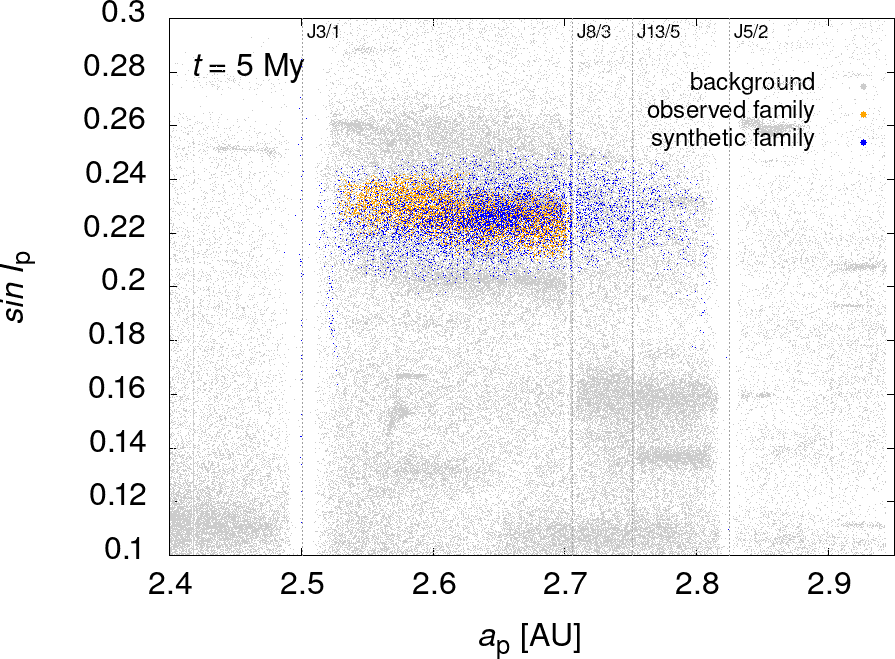
\includegraphics[width=0.49\textwidth]{obr/ai_5t.png}
	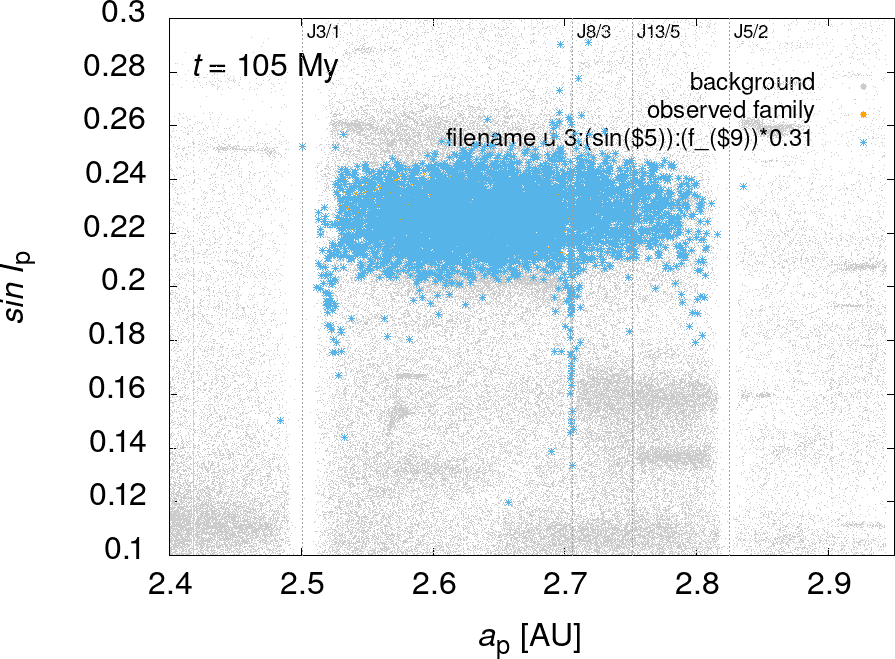
\includegraphics[width=0.49\textwidth]{obr/ai_105t.png}\\
	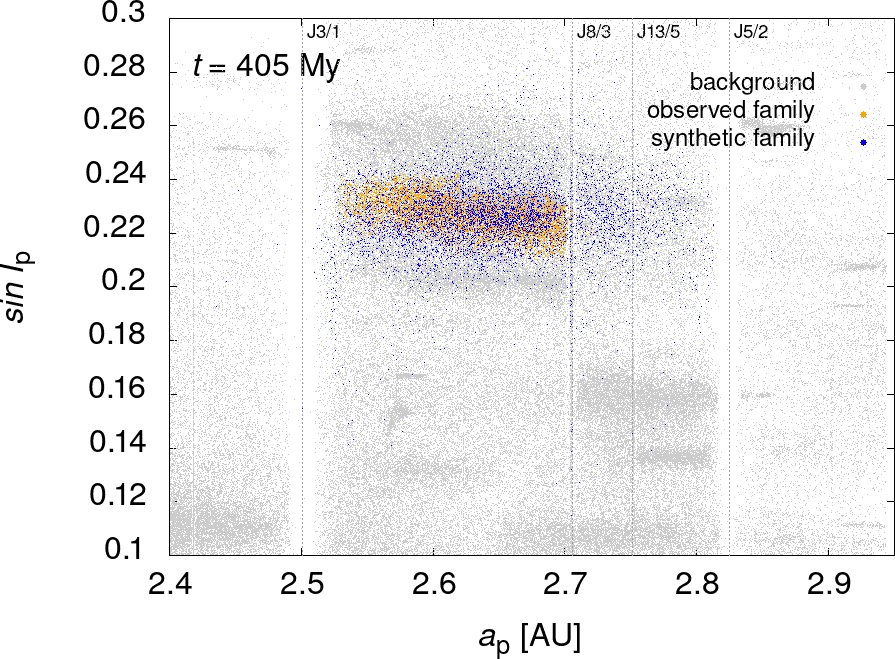
\includegraphics[width=0.49\textwidth]{obr/ai_405t.png}
	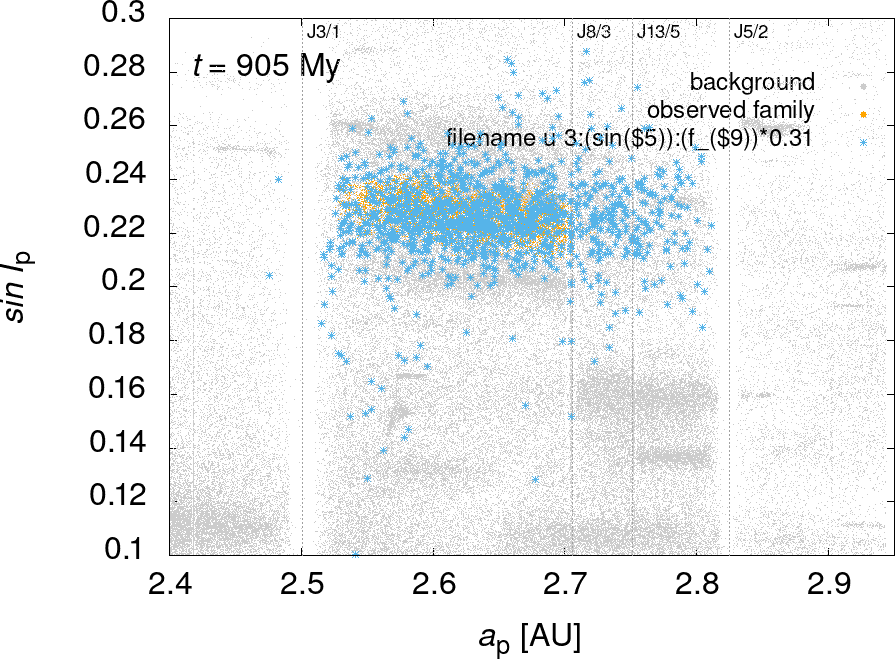
\includegraphics[width=0.49\textwidth]{obr/ai_905t.png}
	\caption{Výsledky simulace v~prostoru $(a_{\rm p},\,\sin I_{\rm p})$ v~časech postupně $t=5,\,105,\,405,\,905$ miliónů let.} \label{fig:ai_sim}
\end{figure}
\immediate\write18{convert -trim obr/ei_5.png obr/ei_5t.png}
\immediate\write18{convert -trim obr/ei_105.png obr/ei_105t.png}
\immediate\write18{convert -trim obr/ei_405.png obr/ei_405t.png}
\immediate\write18{convert -trim obr/ei_905.png obr/ei_905t.png}
\begin{figure}[t]
	\centering
	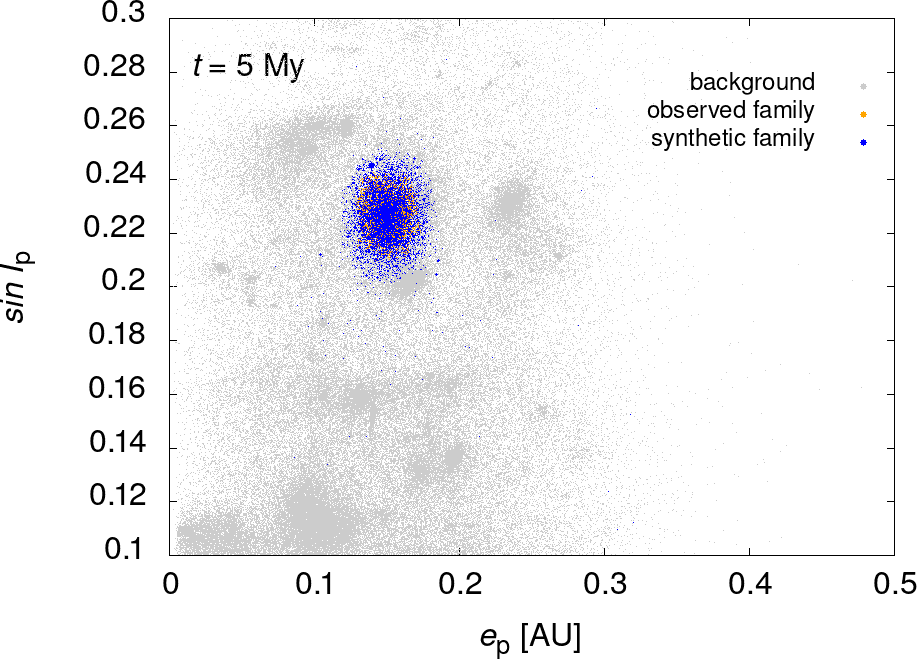
\includegraphics[width=0.49\textwidth]{obr/ei_5t.png}
	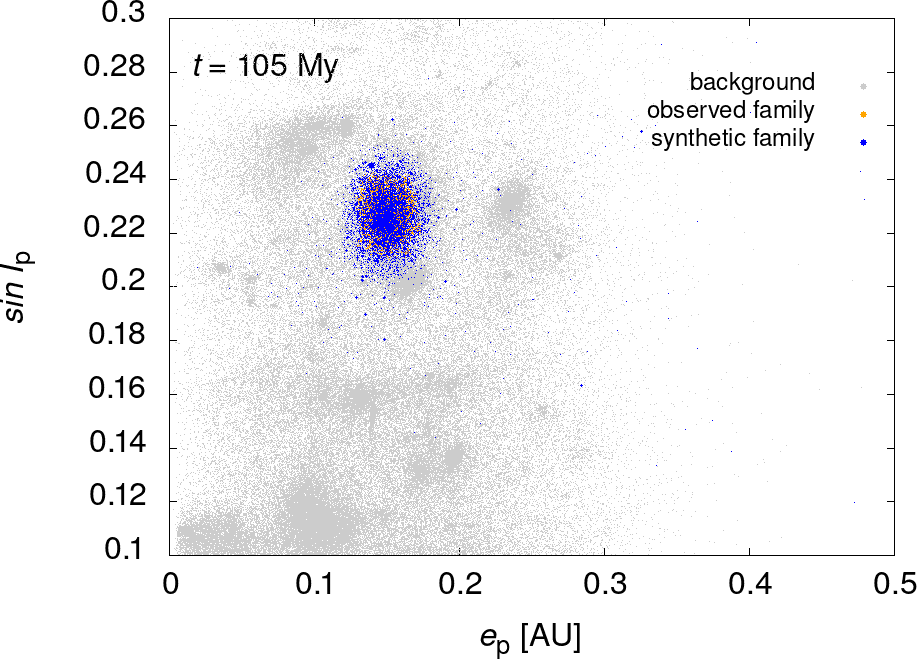
\includegraphics[width=0.49\textwidth]{obr/ei_105t.png}\\
	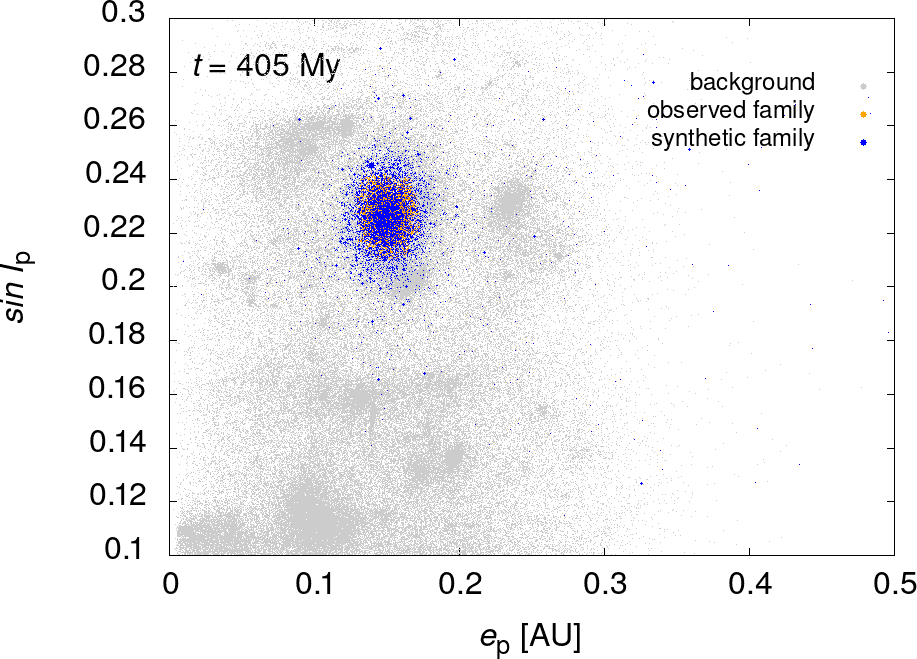
\includegraphics[width=0.49\textwidth]{obr/ei_405t.png}
	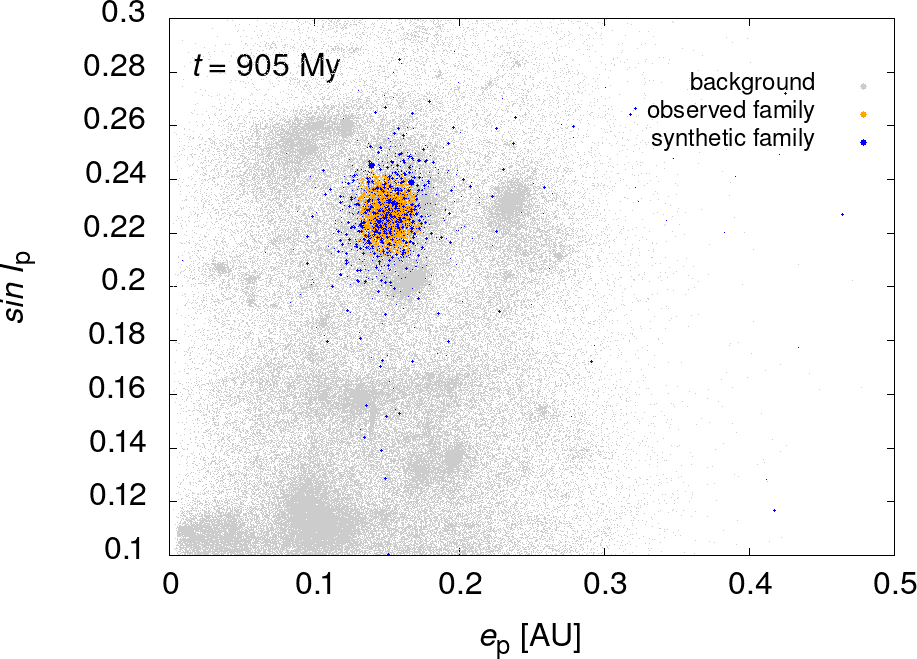
\includegraphics[width=0.49\textwidth]{obr/ei_905t.png}
	\caption{Výsledky simulace v~prostoru $(e_{\rm p},\,\sin I_{\rm p})$ v~časech postupně $5$, $105$, $405$ a~$905$ miliónů let. Fialový obdélník označuje oblast vybranou pro vzorek populace pozadí.} \label{fig:ei_sim}
\end{figure}

Na následujících obrázcích \ref{fig:ae_sim} až $\ref{fig:ei_sim}$ můžeme vidět simulovanou rodinu Eunomia v~porovnání s~rodinou pozorovanou a~s~pozadím v~prostorech $(a_{\rm p},\,e_{\rm p})$, $(a_{\rm p}, \sin I_{\rm p})$ a~$(e_{\rm p},\,\sin I_{\rm p})$ v~časech postupně $5$, $105$, $405$ a~$905$ miliónů let. Z~důvodu velkého objemu dat byly výstupní soubory průměrovány po $10$ milionech let metodou klouzavého okna\footnote{Jednoduše řečeno se pro každou planetku v~nepřekrývajících se časových intervalech o~délce $10$ miliónů let spočetl aritmetický průměr hodnot elementů dráhy a~tyto průměry byly uloženy do nového souboru s~časovým údajem v~půlce intervalu (proto začínáme na $5$ miliónech let)}

Úvodní rozpad v~simulaci byl izotropní, ale kvůli specifickému výpočtu vlastních elementů dráhy z~počátečních rychlostí pomocí Gaussových rovnic můžeme v~čase $t=5$ miliónů let pozorovat mírně nesymetrický tvar simulované rodiny. Dále si můžeme všimnout, že počáteční rodina je o~něco větší než rodina pozorovaná, což nám ale nevadí, protože vždy můžeme vybrat libovolnou podmnožinu planetek, neboť testovací částice spolu neinteragují.

Můžeme pozorovat vliv rezonancí --- u~těch nejsilnějších (J3/1 a~J5/2) se planetky nejvíce vychylují, když se nacházejí v~oblasti separatrixy (šikmá hranice \uv{před} a~\uv{za} rezonancí), načež se jejich excentricity začnou zvyšovat, až se dostanou do oblasti, kde kříží dráhy Marsu nebo Jupitera, což znamená, že se planetka dříve nebo později některé z~těchto planet přiblíží a~její velká poloosa se náhle změní. U~rezonance J3/1 lze vidět u~některých těles naopak pokles excentricity, to ale může být důsledek specifického výpočtu vlastních elementů dráhy, které bývají ovlivněné blízkostí rezonance.

Kromě těchto dvou rezonancí je patrný vliv rezonancí vyšších řádů --- J8/3 a~J13/5 jasně rozdělují planetky simulované rodiny Eunomia do oblastí mezi rezonancemi, ze kterých planetky zřídkakdy vystupují. Vzhledem k~tomu, že na prvním obrázku jsou průměrovaná data z~prvních $10$ miliónů let, můžeme vidět, že se planetky, které se zřejmě od počátku nacházely v~blízkosti rezonancí J3/1, J8/3 a~J13/5, stihly rozptýlit a~narušily tak jinak zatím pravidelný tvar rodiny. Dále se potvrzuje, že rezonance J8/3 je silnější než rezonance J13/5, protože se planetky v~její blízkosti v~čase $t=105$ miliónů let rozšířily do pásu o~velikosti $0,05<e_{\rm p}<0,5$, zatímco v~blízkosti rezonance J13/5 pouze do pásu o~velikosti $0,1<e_{\rm p}<0,23$.

V~populaci pozadí si můžeme všimnout velice slabé rezonance na $a\approx2,62\,{\rm AU}$ a~$2,66\,{\rm AU}$ --- jejich působení na simulované rodině nemůžeme pozorovat na obrázcích v~tištěné práci, lze ale jejich slabý vliv pozorovat při procházení všech obrázků z~celé simulace.

Jednou z~nezodpovězených otázek týkajících se rodiny Eunomia je, zda nepokračuje až za rezonancí J5/2 na $a\approx2,82\,{\rm AU}$~\cite{nesvorny15}. Tento návrh můžeme i~z~této částečné simulace spíše vyvrátit, protože planetky rezonanci J5/2 až na jednotlivé výjimky (viz obrázek ~\ref{fig:ae_sim} pro $t=405\,{\rm My}$) nepřeskakují, ale jsou jí vychylovány až do oblastí křížení drah Marsu nebo Jupitera.

Na obrázcích $(a,\,\sin I_{\rm p})$ lze znovu spatřovat působení rezonancí, tentokrát s~účinkem zvyšování sklonů. Ačkoliv jádro simulované rodiny se zdá v~souladu s~pozorovanou rodinou, můžeme pozorovat mírné \uv{naklonění} pozorované rodiny (část pod $a\approx2,62\,{\rm AU}$ má vyšší sklon $I_{\rm p}$), čehož si na rodině simulované všimnout zatím nemůžeme; tento jev se nám tedy nepodařilo vysvětlit.

Obrázek~\ref{fig:ei_sim} prostoru $(e_{\rm p},\sin I_{\rm p})$ je hlavně zajímavý tím, že na něm jsou jasně vidět okolní rodiny a~jak dochází ke kontaminaci jejich členů s~členy rodiny Eunomia. Také proto byl tento obrázek použit k~vybrání vzorku populace pozadí pro výpočet stáří v~následující kapitole.

\newpage
\section{Odhad stáří}

\immediate\write18{convert -trim obr/ae_chi_0006.png obr/ae_chi_0006t.png}
\immediate\write18{convert -trim obr/ae_chi_0106.png obr/ae_chi_0106t.png}
\immediate\write18{convert -trim obr/ae_chi_0406.png obr/ae_chi_0406t.png}
\immediate\write18{convert -trim obr/ae_chi_empty.png obr/ae_chi_emptyt.png}
\begin{figure}
	\centering
	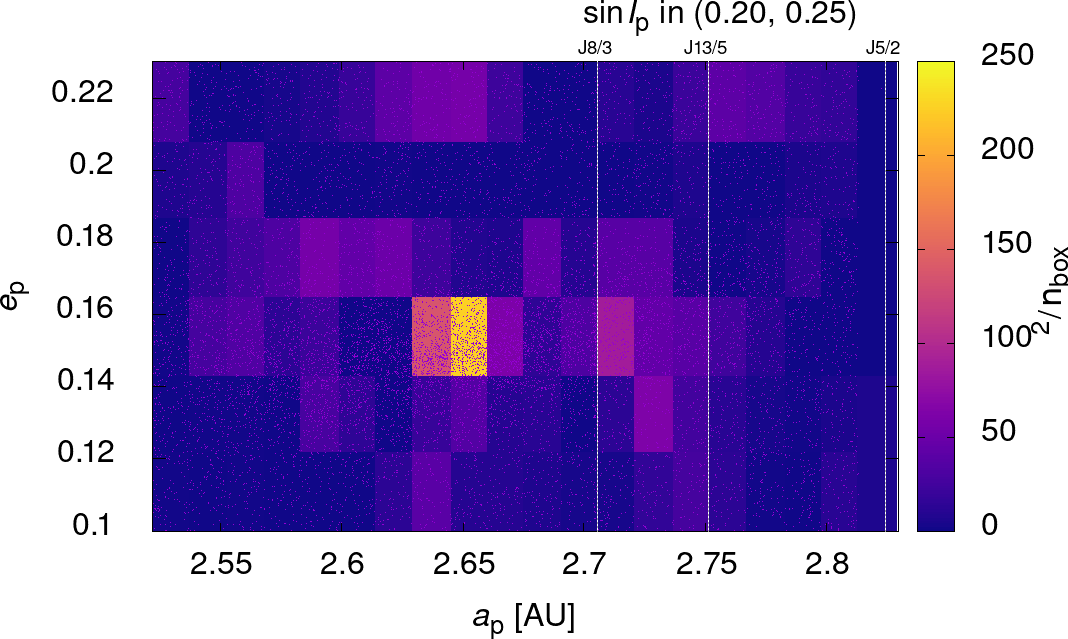
\includegraphics[width=0.49\textwidth]{obr/ae_chi_0006t.png}
	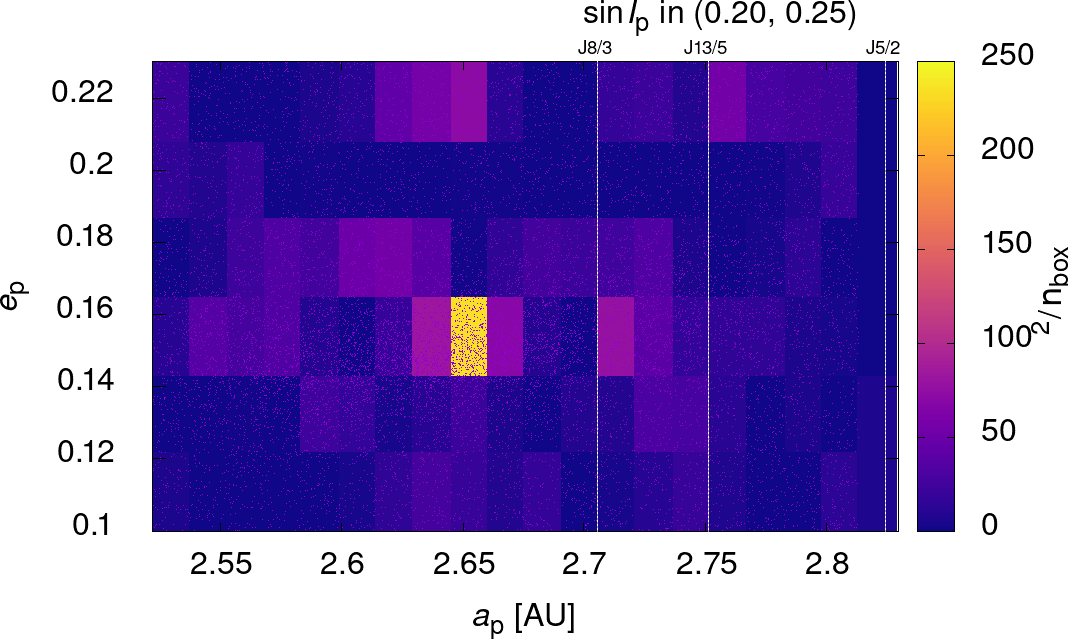
\includegraphics[width=0.49\textwidth]{obr/ae_chi_0106t.png}\\
	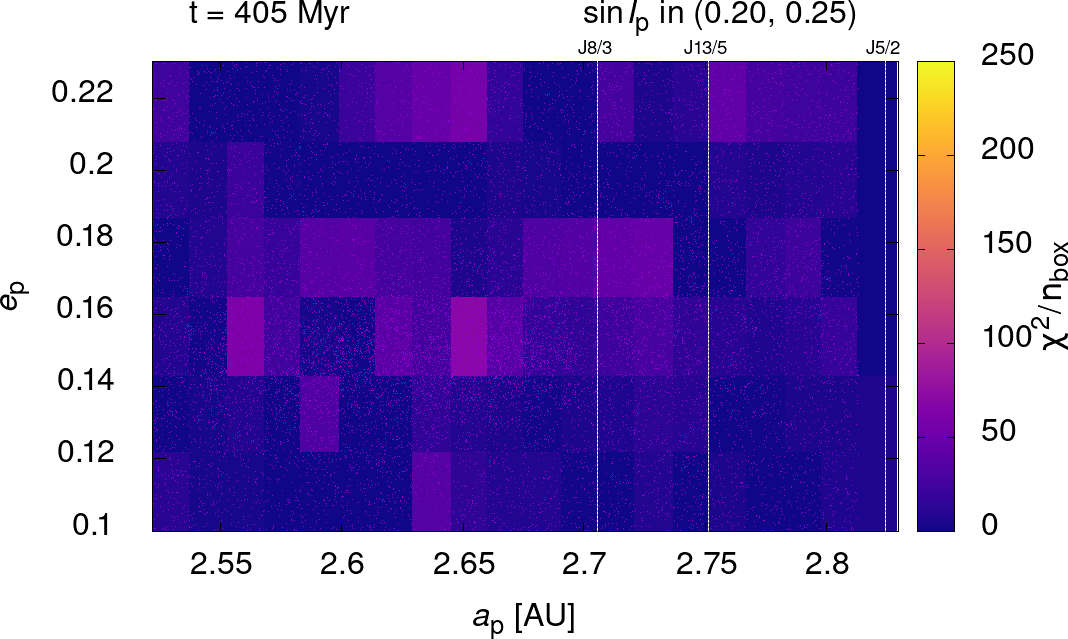
\includegraphics[width=0.49\textwidth]{obr/ae_chi_0406t.png}
	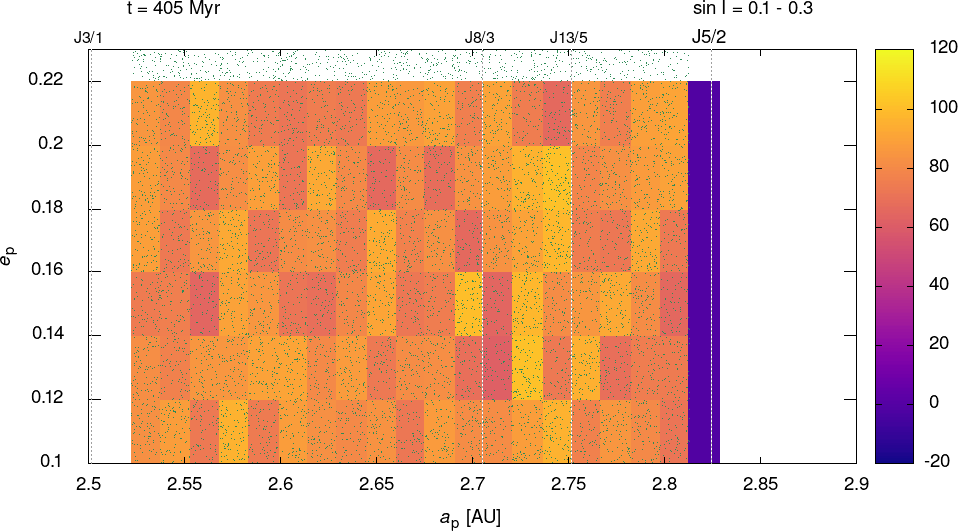
\includegraphics[width=0.49\textwidth]{obr/ae_chi_emptyt.png}
	\caption{Hodnota chi kvadrátu $\chi^2$ pro každý box v~prostoru $(a,\,e)$. Na prvních třech obrázcích lze vidět rozdělení chi kvadrátu pro $t=5,\,105,\,405$ miliónů let, na posledním obrázku lze vidět rozdělení chi kvadrátu při vygenerování pouze pozadí bez použití částic simulované rodiny. Barevná škála je pro všechny až na poslední obrázek stejná. Zelené tečky označují simulovanou populaci i~s~přidaným pozadím. J8/3, J13/5 a~J5/2 označují rezonance středního pohybu s~Jupiterem.} \label{fig:ae_chi2}
\end{figure}

K~odhadu stáří rodiny jsme použili metodu nazvanou příznačně \uv{\textit{blackbox}} popsanou v~\cite{broz19}, která funguje na principu rozdělení planetek jak pozorované, tak simulované rodiny do \uv{boxů} v~prostoru $(a_{\rm p},\,e_{\rm p},\,\sin I_{\rm p})$ a~následném porovnání počtů pozorovaných a~simulovaných planetek v~jednotlivých boxech. Na tento jednoduchý princip je pak použita standardní statistická metoda rozdělení chí kvadrátu $\chi^2$ --- pro každý box vypočteme jeho příspěvek k~ $\chi^2$ jako
\begin{align}
	\frac{(N_{\rm sim}-N_{\rm obs})^2}{N_{\rm sim}+N_{\rm obs}}\,,
\end{align}
kde $N_{\rm sim}$, resp. $N_{\rm obs}$ označuje počet simulovaných, resp. pozorovaných těles v~daném boxu. Dělení výrazem $N_{\rm sim}+N_{\rm obs}$ zohledňuje nejistoty a~zároveň zabraňuje extrémním příspěvkům boxů, kde se $N_{\rm obs}\rightarrow 0$. Výslednou hodnotu $\chi^2$ potom dostaneme prostým sečtením všech příspěvků.

\immediate\write18{convert -trim obr/ae_scl.png obr/ae_sclt.png}
\immediate\write18{convert -trim obr/ae_obs.png obr/ae_obst.png}
\begin{figure}
	\centering
	\includegraphics[width=0.49\textwidth]{obr/ae_scl.png}
	\includegraphics[width=0.49\textwidth]{obr/ae_obs.png}\\
	\caption{Graf $(a_{\rm p}, e_{\rm p})$ pro simulovanou (vlevo) a~pozorovanou (vpravo) rodinu Eunomia v~čase $t=455$ miliónů let, kdy byla hodnota $\chi^2$ nejlepší. Tentokrát barevná škála označuje počet těles v~daném boxu. Lze porovnat s~podobným grafem $\chi^2$ --- problémové oblasti jsou přímo v~centru rodiny (simulovaná populace je příliš kompaktní) a~potom v~oblasti $a_{\rm p}\in(2,55\,{\rm AU};\,2,5\,{\rm AU})$ a~$e_{\rm p}\in(0,14;\,0,16)$, kam se naopak částice simulované populace nestihly rozšířit.} \label{fig:ae_obs_scl}
\end{figure}

Prvním krokem k~provedení této metody je volba samotných boxů. Protože se oblast mezi rezonancemi J8/3 a~J13/5 zdá být pro určení stáří rodiny velmi významná, zvolili jsme boxy tak, aby se v~hlavní poloose mezi tyto rezonance vešly přesně tři. Dále jsme přidali $12$ boxů nalevo a~$5$~napravo, to znamená, že spodní hranice celé oblasti je přibližně před rezonancí J3/1 a~horní přibližně před rezonancí J5/2. V~ostatních elementech jsme hranice zvolili tak, aby pokud možno nenastala kontaminace planetkami okolních rodin. Celkově jsme tedy boxy definovali takto:

\begin{center}
\begin{tabularx}{0.8\textwidth}{|X||c|c|c|}
	\hline
	& Spodní mez & Horní mez & Velikost  \\
	\hline \hline
	Vlastní hlavní poloosa $a_{\rm p}$ & $2,522\,{\rm AU}$ & $2,844\,{\rm AU}$ & $0,0153\,{\rm AU}$ \\
	\hline
	Vlastní excentricita $e_{\rm p}$ & $0,1$ & $0,23$ & $0,0217$ \\
	\hline
	Vlastní sklon $\sin I_{\rm p}$ & $0,2$ & $0,25$ & $0,05$ \\
	\hline
\end{tabularx}
\end{center}

Kvůli nezanedbatelné kontaminaci rodinou Adeona byly její členové ze vzorku pozorované populace ručně odebráni, čímž se výrazně zlepšily naše výsledky. 

Dalším krokem je volba populace pozadí, kterou vybereme z~pozorovaných dat a~\uv{smícháme} ji se simulovanou rodinou tak, aby byl celkový počet syntetických planetek srovnatelný s~celkovým počtem pozorovaných planetek. Jako populaci pozadí jsme po analýze obrázku~\ref{fig:ei_sim} vybrali populaci s~$2,5\,{\rm AU}< a_{\rm p} < 2,7\,{\rm AU}\,, 0,19 < e_{\rm p} < 0,22\,, 0,2 < \sin I_{\rm p} < 0,25$. Princip je takový, že vezmeme pouze rozdělení velikostí planetek z~vybraného pozadí a~náhodně generujeme planetky v~celém objemu, přičemž zachováváme koncentraci těles. Pak doplníme počet planetkami ze simulace rodiny tak, aby se celkový počet vyrovnal počtu pozorovaných planetek o~dané velikost. V~blízkosti rezonance J5/2 jsme žádná tělesa pozadí nevybírali, protože v~realitě je tento prostor víceméně prázdný, kvůli působení rezonance, takže rovnoměrné rozprostírání těles pozadí do toho prostoru by nedávalo smysl.

\begin{figure}
	\centering
	\includegraphics[width=0.7\textwidth]{obr/chi2.eps}
	\caption{Závislost redukovaného chí kvadrátu $\chi^2/n_{\rm box}$ na čase $t$. Lze vidět, že se jeho hodnota snižuje, tudíž můžeme předpokládat, že bychom delší integrací dostali nižší hodnoty, případně bychom mohli určit interval stáří rodiny Eunomia.} \label{fig:chi2}
\end{figure}

Na obrázku~\ref{fig:ae_obs_scl} můžeme vidět simulovanou a~pozorovanou rodinu Eunomia v~okamžiku, kdy jsme dostali nejmenší hodnotu $\chi^2=11,9$, tedy naše data se nejvíce přibližovala realitě. Stále lze ale pozorovat nějaké nedostatky, kromě těch zmíněných v~popisku obrázku můžeme poukázat na oblast $a_{\rm p}\in(2,7\,{\rm AU};\,2,75\,{\rm AU}),\ e_{\rm p}\in(0,16;\,0,18)$, kde se nachází velmi malá rodina příslušná planetce $(53546)\ 2000\,BY6$~\cite{milani14}, se kterou jsme v~naší simulaci, stejně jako s~ostatními menšími rodinami, nepočítali.

Simulovaná rodina se očividně vyvíjí správným směrem ($\chi^2$ klesá) a~lze očekávat, že při delší simulaci bychom dostali nějakou minimální hodnotu $\chi^2$, díky které bychom mohli přesněji určit stáří této rodiny, nicméně prozatím můžeme říct, že rodina Eunomia je pravděpodobně starší než půl miliardy let.

\chapter*{Závěr} \label{ch:zaver} \addcontentsline{toc}{chapter}{Závěr}
V~této práci byl nejprve podán určitý základ k~pochopení výzkumu --- tzn. vysvětlení problému dvou těles, problému $N$ těles, numerického řešení pohybových rovnic, stejně jako pojmů oskulační, střední a~vlastní elementy. Pro podrobnější vysvětlení lze čerpat např. ze zdrojů~\cite{murray00} nebo~\cite{fmt}. Dále jsme představili koncept rodin planetek a~popsali základní metody pro~jejich identifikaci a~analýzu --- některé z~nich jsme poté aplikovali na významnou početnou rodinu středního pásu Eunomia.

Hlavním metodou našeho zkoumání rodiny Eunomia byla její simulace v~$N$ částicovém integrátoru SWIFT, který se k~tomuto účelu používá~\cite{levison94} \cite{broz11}. V~této práci jsme se omezili na možnost vysvětlení rodiny Eunomia jako mladé rodiny --- simulovali jsme tedy přesně 6210 částic, což je srovnatelné se~stávajícím počtem členů pozorované rodiny Eunomia, po dobu 1 miliardy let. Protože data v~časovém úseku $500$ až $1000$ miliónů let stále nebyla kompletní, zaměřili jsme se na úsek $0$ až~$500$ miliónů let a~provedli jsme analýzu rodiny pomocí statistické metody.

K~výpočtu veličiny $\chi^2$ (chí kvadrát) jsme nejprve vybrali vhodnou oblast pro vzorek pozadí v~střední části hlavního pásu planetek, který jsme pak přidali k~simulovaným částicím a~vytvořili tím syntetickou populaci, početně zcela srovnatelnou s~pozorovanými daty ve~zvolené oblasti. Při analýze jsme narazili na několik překážek, které jsme museli překonat, jako například kontaminace ostatními rodinami. Takto se nám podařilo vysvětlit většinu struktur, které lze na našich grafech vlastní velké poloosy $a_{\rm p}$, vlastní excentricity $e_{\rm p}$ a~vlastního sklonu $I_{\rm p}$ pozorovat. Jediné, co zůstává nevysvětlené, je kompaktnost jádra simulované rodiny a~absence částic ve~oblasti \uv{nalevo} ($a_{\rm p}<2,57\,{\rm AU}$) od středu rodiny na grafu $(a_{\rm p},\,e_{\rm p})$. Tyto jevy bohužel musíme připsat nedostatečně dlouhému časovému úseku, po který jsme rodinu Eunomia simulovali --- velice pravděpodobně tedy rodina Eunomia není mladší než $500$ miliónů let.

Na grafu $\chi^2$ v~závislosti na čase $t$ bylo ovšem možné pozorovat klesající trend, což znamená, že pokud bychom v~budoucnu simulovali rodinu Eunomia po celé 4 miliardy let, zřejmě bychom dostali nějakou minimální hodnotu $\chi^2$, čímž bychom přesněji určili její stáří. Další možnosti výzkumu jsou analýzy okolních rodin, zejména rodiny Adeona, která naši rodinu Eunomia značně kontaminuje. Přesné určení počtu jejích rozptýlených členů a~stáří by nám velmi pomohlo v~analýze rodiny Eunomia, mohli bychom například v~momentu rozpadu rodiny Adeona její částice přidat do simulace.

Po prodloužení dlouhodobé simulace plánujeme publikaci výsledků v~odborném časopisu (\textit{Icarus}).

%{{{ Bibliografie
\newpage

\printbibliography
%}}}
%{{{ Přílohy
\begin{appendices}
	\chapter{Ilustrace Eulerovy metody ve~vektorové grafice} \label{app:asy}
	\begin{figure}[!htb]
	\centering
	\asyinclude{f_euler.asy}
	\end{figure}

	K~vytvoření ilustrace Eulerovy metody na obrázku~\ref{fig:euler} byl použit vektorový grafický jazyk \textit{Asymptote}, který je svým způsobem následovníkem staršího a~dosud také velmi využívaného \textit{MetaPostu}. Svou syntaxí se podobá jazyku $C++$ a~ke generování popisků a~značek používá \LaTeX. Výstup je ve~formátu \textit{PostScript}, ale lze ukládat i~do PDF.

\lstinputlisting[language=Gnuplot]{asy/f_euler.asy}

	\chapter{Výpočet Keplerovy rovnice pomocí iterační metody} \label{app:kepit}
	Kód na výpočet Keplerovy rovnice, viz~\eqref{eq:kepler}, v~programovacím jazyce \textit{Python} pomocí iterační metody, jejímž předpisem je
	\begin{align*}
		E_{i+1}=M+e\sin{E_i}q\,, \quad \text{pro}\ i=0,\,1,\,2,\,\ldots
	\end{align*}
	kde bereme první odhad $E_0=M$. Algoritmus ukončíme, když dosáhneme přesnosti ${eps<10^{-13}}$, což odpovídá dvojité přesnosti reálných čísel v~dnešních standardních programovacích jazycích.

	Tato metoda konverguje k~řešení pouze pro excentricity $e<0,6627434\,$, pro vyšší excentricity je nutné využít jiné numerické metody.
\begin{lstlisting}[language=Python]
from math import sin

def kepler(M, e):
    """Solution of Kepler align"""
    eps = 1E-13
    E2 = M + e*sin(M)
    while True:
        E1 = E2
        E2 = M + e*sin(E1)
        if abs(E2 - E1) < eps:
            break 
    return E2
\end{lstlisting}
	\chapter{Výpočet polohy tělesa z~oskulačních elementů} \label{app:el2xyz}
\vspace{-36pt}
\begin{enumerate}[label=\arabic*.]
	\item Z~Keplerovy rovnice \eqref{eq:kepler} některou ze jmenovaných metod (aproximační, iterační nebo numerickou) vypočítáme velikost excentrické anomálie $E$ ze střední anomálie $M$.
	\item Vztah \eqref{eq:fE} upravíme a~spočteme pravou anomálii $f$
		\begin{align}
			f = 2\arctg\left(\sqrt{\frac{1+e}{1-e}}\tg \frac{E}{2}\right)\,.
		\end{align}
	\item Pomocí vztahu 
\vspace{-12pt}
		\begin{align}
			r=a(1-e\cos E)\,,
		\end{align}
		vypočítáme velikost $r$ --- relativní vzdálenost tělesa od Slunce.
	\item Pomocí vztahů
\vspace{-12pt}
		\begin{align}
			x&=r\left[\cos\Omega\cos(\omega+f)-\sin\Omega\sin(\omega+f)\cos i\right]\,, \\
			y&=r\left[\sin\Omega\cos(\omega+f)+\cos\Omega\sin(\omega+f)\cos i\right]\,, \\
			z&=r\sin i\sin(\omega+f)\,,
		\end{align}
		vypočítáme $x,\,y,\,z$.
\end{enumerate}
	\vspace{-12pt}
	Dále můžete nalézt kód na tento výpočet v~jazyce \textit{Python}, který byl použit například na vygenerování obrázku krátkodobé simulace~\ref{fig:trajec}. Vstupním souborem je \I{bin.out}, což je výstupní soubor integrátoru SWIFT (nutno však nejprve použít program \I{follow2} na získání dat z~binárního souboru $bin.dat$), který má formát prostého textu, kde jsou jednotlivé sloupce oddělené tabulátory. Výstup programu je ve~formátu $t\,[{\rm Yr}]\ x\,[{\rm AU}]\ y\,[{\rm AU}]\ z\,[{\rm AU}]$ a~lze ho použít pro vygenerování animace jako v~\ref{fig:trajec} pomocí nějakého grafovacího programu, např. \textit{Gnuplotu}.
	\begin{lstlisting}[language=Python]
from math import *

def el2xyz(path):
    """Conversion from orbital elements to xyz positions (from text file bin.out by program follow2)"""
    binout = open(path, 'r')
    for line in binout.readlines()
        l = line.split()
        id = int(l[0])
        if id > 0:
            t = float(l[1])
            a~= float(l[2])
            e = float(l[3])
            inc = radians(float(l[4]))
            capom = radians(float(l[5]))
            omega = radians(float(l[6]))
            M = radians(float(l[7]))
    
            # Note: The approximation by 3 terms was not sufficient
            # E = M + (e-pow(e,3.0)/8.0)*sin(M) + pow(e,2)/2.0*sin(2.0*M) + pow(e,3)*3.0/8.0*sin(3.0*M)
            E = kepler(M, e)
            f = 2.0*atan(sqrt((1.0+e)/(1.0-e))*tan(E/2.0))
            r = a*(1-e*cos(E))
            x = r*(cos(capom)*cos(omega+f)-sin(capom)*sin(omega+f)*cos(inc))
            y = r*(sin(capom)*cos(omega+f)+cos(capom)*sin(omega+f)*cos(inc))
            z~= r*sin(inc)*sin(omega+f)
            print (t + " " + str(x) + " " + str(y) + " " + str(z))

def main():
    if (len(sys.argv) >= 2):
        el2xyz(sys.argv[1])
    else:
        print "Usage el2xyz.py infile"

if __name__ == "__main__":
    main()
	\end{lstlisting}

	\chapter{Skripty k~vytvoření obrázků $(a,\,e)$} \label{app:fig:ae_sim}
	K~vytvoření jednotlivých souborů pro vytvoření grafů je neprve potřeba setřídit data z~integrátoru podle času --- počátečně jsou totiž seřazeny podle jednotlivých skupin po 200 částicích. Následující skript v~jazyce \textit{Python} má jako vstup již sloučený a~po 10 miliónech let zprůměrovaný soubor \textit{bin.proper10My.out} a~jeho výstupem jsou rozdělené soubory podle časových okamžiků ve~složce \textit{split/} ve~tvaru \textit{bin.proper10My.out\_time\_sorted[n]}.
	\begin{lstlisting}[language=Python]
#!/usr/bin/env python
# Roztridit data z~integratoru SWIFT podle cau
__author__ = "Adam Krivka"

import operator

# Nacteni dat
fin = open("bin.proper10My.out", "r")
data = fin.readlines()
ddat = open("D.dat", "r") # prumery castic
genvel = open("genvel3.out_v", "r") # rychlosti castic po rozpadu

# definice promennych
ids = {}
times = {}
d = dict(enumerate(ddat.readlines(),1))
v~= dict(enumerate(genvel.readlines(),1))

id_offset = 0
t_prev = 0

# nacteni dat do promennych (dictionary)
for i, line in enumerate(data):
    iid = int(line.strip().split()[0])
    t = float(line.strip().split()[1])

    if t < t_prev:
        id_offset += 200
    t_prev = t

    times[i] = int(t) # zaokrouhlujeme
    ids[i] = iid+id_offset

n = 1
prev_id = 2
fout_time = open("split/bin.proper10My.out_time_sorted" + str(n), "w")

# samotne setrizeni
for i, t in sorted(times.items(), key=operator.itemgetter(1)):
    if ids[i] < prev_id:
        fout_time.close()
        fout_time = open("split/bin.proper10My.out_time_sorted" + str(n), "w")
        n += 1
    prev_id = ids[i]

    # ukladani dat vcetne prumeru a~rychlosti
    out = data[i].replace(data[i].strip().split()[0], str(ids[i]), 1).strip() + "   " + d[ids[i]].strip() + " " + v[ids[i]].strip()
    fout_time.write(out.strip() + "\n")

fin.close()
	\end{lstlisting}
	
	K~vytvoření samotného obrázku (a~ostatně i~většiny grafů v~této práci) jsme použili volně dostupný grafovací program \textit{Gnuplot}. Následující skript vytváří obrázek~\ref{fig:ae_sim} v~prostoru $(a,\,e)$ a~externě jsou mu vkládany hodnoty proměnných \textit{amin}, \textit{amax}, \textit{emin}, \textit{emax} a~\textit{filename}, přičemž poslední z~nich je cesta k~souborům ve~tvaru \textit{bin.proper10My.out\_time\_sorted[n]}, vytvořené předešlým skriptem v~\textit{Pythonu}. Ostatní proměnné a~jiné grafické prvky jsou načteny ze souboru \textit{preamble.plt}.

\begin{lstlisting}[language=Gnuplot]
#!/usr/bin/gnuplot

%load "preamble.plt"

set xlabel "{/Helvetica-Oblique a}_p [AU]"
set ylabel "{/Helvetica-Oblique e}_p"

set xrange [amin:amax]
set yrange [emin:emax]

e(a,q)=abs((q-a)/a)

plot 	"check_BOX.dat" using 36:37:(f_(D($35,p_V))*0.3) with point linestyle 1 pointsize variable linecolor rgb "0xcccccc" title "background",\
 	"eunomia_family.list" using 36:37:(f_(D($35,p_V))*0.3) with points linestyle 2 pointsize variable title "observed family",\
	filename using 3:4:(f_($9)*0.31) with points title "synthetic family" linestyle 3 pointsize variable,\
	e(x,1.52) not linetype 8 linewidth 1
quit
\end{lstlisting}
\end{appendices}
%}}}
\end{document}
